Ein wesentlicher Aspekt der K.I.\ ist es die aktuelle Spielfeldsituation der unterschiedlichen Spieler zu bewerten.
Dadurch kann die K.I.\ Spielz\"uge besser einstufen und gegebenenfalls das Spiel mit Spezialsteinen beeinflussen.
Ein naiver Ansatz w\"are der Vergleich der Anzahl an Spielsteinen jedes Spielers.
Dieses Vorgehen reicht jedoch nicht f\"ur eine ad\"aquate Bewertung der Spielsituation aus.
In Abbildung~\ref{fig:naivespielfeld01} w\"urde die naive Vorgehensweise den roten Spieler besser einstufen, jedoch hat er hier keinerlei m\"ogliche Spielz\"uge.
Der rote Spieler kann trotz dieser \"Uberlegenheit nicht mehr gewinnen, da der blaue Spieler im n\"achsten Spielzug \"uber alle roten Steine hinwegziehen kann.
Genau aus diesem Grund reicht eine naive Spielfeldbewertung nicht f\"ur ein aussagekr\"afigtes Resultat aus.

\vspace{1em}
\begin{minipage}{\linewidth}
    \centering
    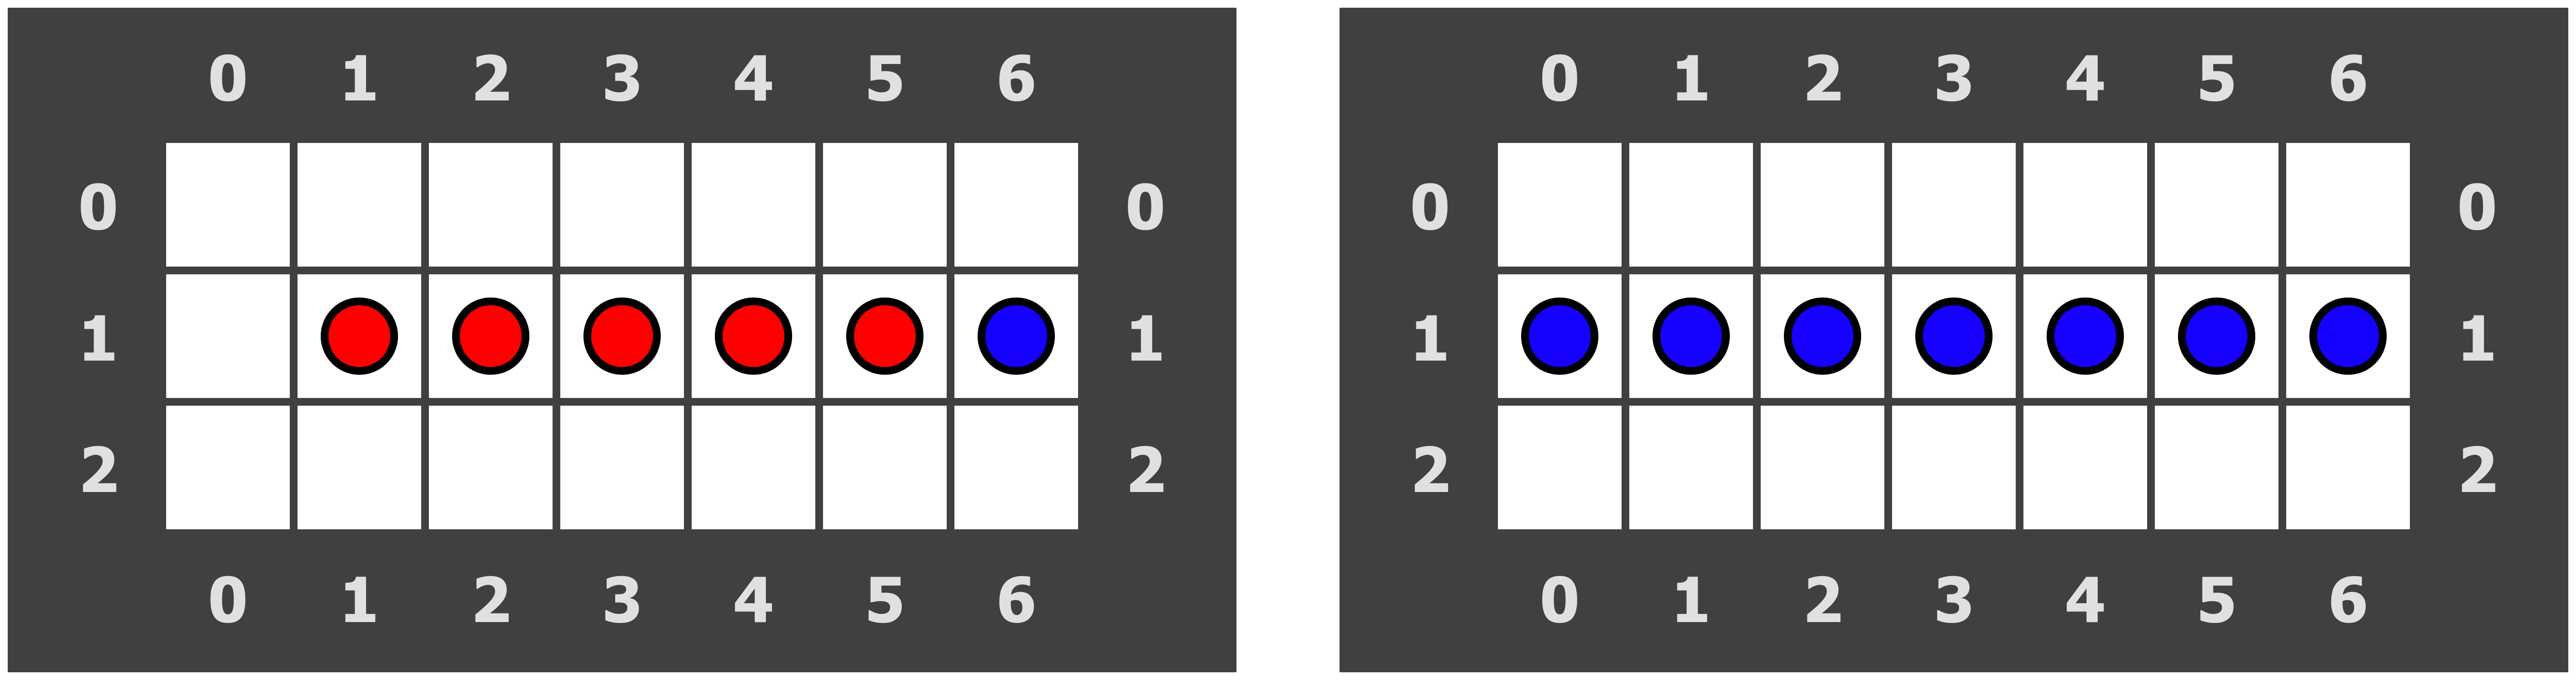
\includegraphics[width=0.6\linewidth]{pics/naive-game-situation}
    \captionof{figure}{Problematik der naiven Bewertung}
    \label{fig:naivespielfeld01}
\end{minipage}

\subsection{Bestandteile der Heuristik}\label{subsec:bestandteile-der-heuristik}
Wie bereits in der Einleitung dieses Abschnitts begr\"undet, gen\"ugt das reine Abz\"ahlen der Spielsteine nicht aus.
Deshalb setzt dieser Client auf drei unterschiedliche Heuristikbestandteile, um die aktuelle Spielsituation zu bewerten.
Unter diesen drei Ans\"atzen werden die \emph{Mobilit\"at} der Spieler, das \emph{Verh\"altnis der Spielsteine} sowie die aktuelle \emph{Bewertung der Karte} miteinbezogen.
Diese einzelnen Bestandteile sind w\"ahrend des Spiels jedoch nicht immer gleichbedeutend.
Zu Beginn muss darauf geachtet werden, dass man sehr flexibel bleibt und Positionen erobert die sp\"ater nur schwer einnehmbar sind.
Hierzu z\"ahlen vor allem Ecken und Kanten.
Erobert man nun ein solches Feld, wird der Gegner in seiner Zugwahl eingegrenzt, da er keine Z\"uge w\"ahlen will, die bereits einen Zug sp\"ater wieder \"uberzogen werden.
Eine solche Situation schr\"ankt die Mobilit\"at des Gegners drastisch ein und auch die Bewertung des Spielers aufgrund seines Kartenwertes leidet darunter.
Je weiter man sich jedoch dem Spielende n\"ahert, desto unwichtiger wird dieses Bewertungskriterium.
Dies liegt daran, dass man das Spiel nicht aufgrund hoher Mobilit\"at gewinnt, sondern anhand der Anzahl seiner Spielsteine.
Aus diesem Grund wird das Verh\"altnis der Spielsteine zum Ende hin immer wichtiger.
Ma"sgeblich ist nun den prozentualen Spielverlauf abzusch\"atzen, um damit die einzelnen Heuristikbestandteile akkurat gewichten zu k\"onnen.

\subsubsection{Gewichtung des Spielfeldes}\label{subsubsec:gewichtung-des-spielfeldes}
Die Bewertung der Karte ist eine dynamisch ver\"andernde Heuristik in ReversiXT.
Diese Heuristik ist das Auge des Clients, da nur so begehrenswerte Felder wie Ecken oder Bonussteine erkannt werden k\"onnen und diese enorme Vorteile w\"ahrend des gesamten Spielverlaufes geben.
Ecken und Kanten sind dabei besonders interessant.
Zwar sind sie schw\"acher als im originalen Reversi, da man Sie mit \"Uberschreib-, Choice- oder Inversionsteinen immer noch einnehmen kann.
Trotzdem k\"onnen fr\"uh eingenommene Ecken und Kanten der Grundstein f\"ur ein dominantes Spiel sein und m\"ussen deswegen kontrolliert werden.

\paragraph{Erreichbare Felder}
Bevor die Karte bewertet oder irgendein Zug berechnet wird, kalkuliert der \emph{MapAnalyzer}, welche Felder auf der Karte theoretisch erreichbar sind und welche nicht.
In den n\"achsten Bewertungsschritten werden alle laut MapAnalyzer nicht erreichbaren Felder als Loch gesehen.
F\"ur diese Felder wird an sich kein Wert berechnet, da niemals ein Zug auf Sie stattfinden wird.
Es k\"onnen aber in die Bewertung anderer Felder einbezogen werden, was im nachfolgenden Kapitel beschrieben wird.

\paragraph{Feldbewertung}
\vspace{1em}
\begin{minipage}{\linewidth}
    \centering
    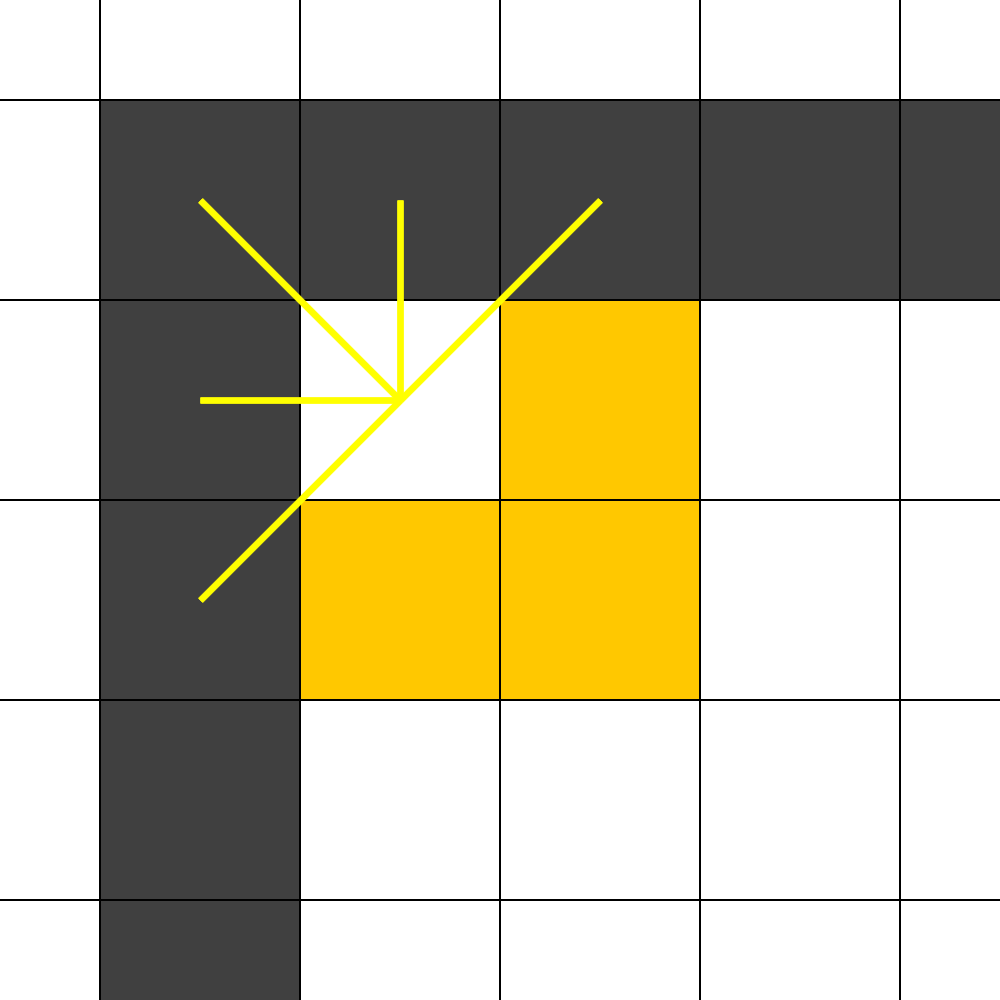
\includegraphics[width=0.2\linewidth]{pics/edge}
    \captionof{figure}{Bild einer Ecke in ReversiXT, mit 5 nicht bespielbaren Feldern.}
    \label{fig:edge}
\end{minipage}
\vspace{1em}

Jedes einzelne erreichbare Feld wird bewertet und erh\"alt einen Grundwert.
Dieser Grundwert berechnet sich aus der Anzahl der nicht erreichbaren Nachbarfelder, multipliziert mit einem festen \emph{Faktor} der die Feldbewertung nochmals anhebt.
Ecken haben so zum Beispiel den Grundwert~$5$, da in ihrem direkten Umfeld f\"unf Felder nicht begehbar sind (siehe Abbildung~\ref{fig:edge}).
Dieser Wert wird anschlie"sen noch mit einem festen Wert multipliziert, der sich f\"ur alle Abstufungen von Ecken \"andert.

\paragraph{Bewertung von Nachbarfeldern}
Bei der Feldbewertung werden nicht nur die Felder an sich bewertet.
Die Bewertung wirkt sich auch auf benachbarte Felder aus.
So kann er Client entscheiden, dass es eventuell nicht sehr schlau ist, direkt neben ein begehrenswertes Feld zu ziehen, und es damit dem Gegner zu erm\"oglichen einfach \"uber einen dr\"uberziehen um dieses Feld zu erobern.
Um dem entgegenzuwirken, beeinflussen Felder auch ihre Nachbarfelder in alle Zugrichtungen.
Das folgende Bild zeigt die Ausbreitung dieser Welle.

\vspace{1em}
\begin{minipage}{\linewidth}
    \centering
    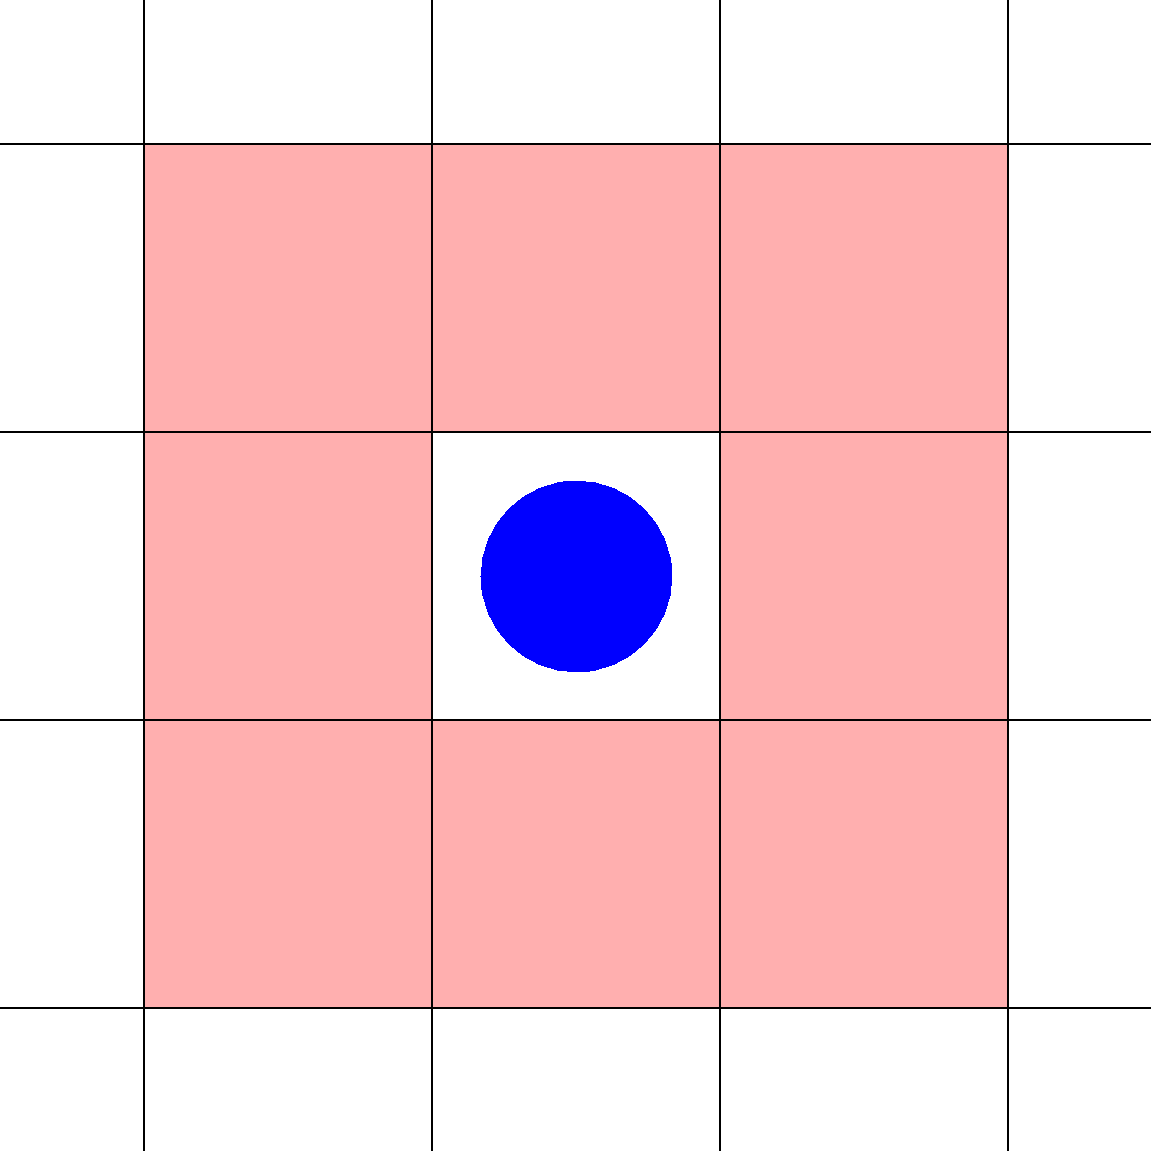
\includegraphics[width=0.2\linewidth]{pics/middle}
    \captionof{figure}{Ausbreitung eines Feldes rot markiert.}
    \label{fig:middle}
\end{minipage}
\vspace{1em}

Das blau markierte Feld ist das zu analysierende Feld.
Alle rot markierten Felder bekommen einen Malus auf ihren Wert.
Somit sind sie f\"ur die Zugberechnung weniger attraktiv.
Das blaue Feld hingegen erh\"alt einen Bonus auf seinen Wert, da man es gerne erreichen m\"ochte.
Diese Welle breitet sich auch \"uber Transitionen hinweg aus.
Des Weiteren wird beim Ziehen auf ein Feld auch die Welle entfernt.
Das ist besonders bei Spezialfeldern wichtig, da sobald dies ausgel\"ost wurden alle Felder im Umkreis wieder \textit{normal} attraktiv sein m\"ussen und keinen Bonus mehr aufgrund des Spezialfeldes ben\"otigen.
Diese Gewichtung wird durch den MapAnalyzer entfernt.

\paragraph{Faktor der Felder}
In ReversiXT sind Ecken sehr viel Wert, doch bei einigen Karten gibt es sehr viele Ecken.
Die Frage ist also, wie man diese einzelnen Ecken unterscheidet und nach Nutzen sortieren kann.
Jede Ecke im Spiel hat einen Faktor der sich daraus berechnet, wie weit man von diesem Feld aus jeweils in eine Richtung gehen kann ohne auf ein Loch zu sto"sen.
Transitionen wird dabei nat\"urlich gefolgt.
F\"ur jedes erreichte Feld wird nun der Faktor von $1.0$ an um $0.1$ erh\"oht.
Die Folge ist, dass Ecken von denen man in verschieden Richtungen weit in die Karte ziehen kann h\"oher bewertet und damit vom Client bevorzugt werden.

\paragraph{Bewertung von Spezialfeldern}
Spezialfelder machen ReversiXT aus.
Sie haben einen enormen Einfluss auf das Spiel und k\"onnen Partien schnell drehen.
Deshalb ist die Kontrolle und Priorit\"at dieser Felder mit Bonussteinen extrem wichtig.
Wie wichtig die einzelnen Bonussteine sind, wurde vom Team gemeinsam in den ersten Stunden beschlossen und folgende Priorit\"at festgelegt:
\begin{align}
    \texttt{Bonusstein} > \texttt{Choice} > \texttt{Inversion}
\end{align}

Der Bonusstein wird periodisiert, da so in den letzten Z\"ugen der ersten Phase nochmals sehr viele Steine umgef\"arbt werden k\"onnen.
Die Bewertung der Bonusfelder ist genau so wie bei einem \textit{normalen} Feld.
Das zu berechnende Feld bekommt je nachdem, ob es ein Choice-, Inversion- oder Bonusfeld ist, einen Bonuswert, der es bei der Zugauswahl extrem attraktiv macht.
Da der Feldwert des Bonusfeldes sehr hoch ist, wirkt sich dies nat\"urlich auf die umstehenden Felder aus, weshalb die angrenzenden Felder dementsprechend unattraktiv sind.
Zus\"atzlich gibt es bei der Bonusfeldbewertung die M\"oglichkeit, Felder als aktiviert zu setzen, wodurch die Welle auf diesem Feld r\"uckg\"angig gemacht wird.
Dies ist n\"otig, um sicherzustellen, dass die K.I.\ nicht durch bereits aktivierte Spezialfelder beeinflusst wird.

\subsubsection{Mobilit\"at}\label{subsubsec:mobilitaet}
Ein weiterer Bestandteil der Analyse besteht darin, Spielsituationen anhand der Beweglichkeit der Spieler einzustufen.
Hierbei wird die Anzahl an Spielz\"ugen eines jeden Spielers bestimmt und miteinander verglichen.
Wie bereits in der Einleitung gezeigt kann ein Spieler seine positive Stellung nur halten, solange er weiterhin spielf\"ahig bleibt.
Aus diesem Grund wird in diesem Ansatz bestimmt wie beweglich ein Spieler gegen\"uber den Anderen ist.

Ein Vorteil dieser Bewertungsmethode besteht darin, dass ein Spieler mit wenig Steinen aber einer hohen Mobilit\"at bei diesem Verfahren nicht negativ bewertet wird.
Ein Problem daran ist jedoch, dass zum Ende des Spieles dieser Ansatz an Relevanz verliert, da zum Schluss nur die Anzahl an eigenen Steinen entscheidend ist.

\subsubsection{Spielfeldbelegung}\label{subsubsec:spielfeldbelegung}
Da es besonders gegen Ende des Spiels essenziell ist, viele Steine zu besitzen, muss man dies ebenfalls in die Bewertung miteinbeziehen.
Anstatt aber nur einfach die Anzahl der Spielsteine zu z\"ahlen, wird hier das prozentuale Verh\"altnis gegen\"uber allen existierenden Spielsteinen genommen.

Der Vorteil dieses Verfahrens ist hier, dass man vor allem im sp\"ateren Spielverlauf feststellen kann, wie der aktuelle Stand des Spiels ist und welche Spieler es anzugreifen gilt.
Der Nachteil hierbei ist aber, dass dieses Verfahren im anf\"anglichen und mittleren Spielverlauf nicht aussagekr\"aftig ist.
Dies liegt daran, dass man besonders zum Spielende durch eine zuvor sehr gute Mobilit\"at einen vermeintlich besseren Spieler sehr viele Steine wegnehmen kann.
Allerdings muss man diese Berechnung wie Anfangs erw\"ahnt mit einflie"sen lassen, da man zum Schluss einen Greedyansatz w\"ahlen muss.
Denn letztlich ist f\"ur das Gewinnen des Spieles nur die Anzahl an Spielsteinen von Bedeutung.

\newpage

\subsection{Algorithmen der Zugauswahl}\label{subsec:algorithmen-der-zugauswahl}
F\"ur einen Computer ist es unm\"oglich den besten Spielzug zu finden, da hier jedes m\"ogliche Spielfeld \"uberpr\"uft werden m\"usste.
Bei einem Spiel wie Schach w\"aren dies circa $10^{120}$ unterschiedliche Spielbrettzust\"ande~\cite{chessBoards}.
Bei ReversiXT liegt die Zahl wesentlich h\"oher, da es zum einen viel gr\"o"sere Karten und zum anderen bis zu 8 Spieler gibt.
Damit ein Computer trotzdem einen guten Zug abliefern kann werden spezielle Algorithmen ben\"otigt.
Ein weit verbreiteter Algorithmus f\"ur Zwei-Personen-Nullsummenspiele\footnote{Duden: Spiel, bei dem die Summe der Eins\"atze, Verluste und Gewinne gleich null ist} lautet Minimax.

\subsubsection{Minimax Algorithmus}\label{subsubsec:minimax-algorithmus}
Zur Veranschaulichung von Minimax soll ein kurzes Gedankenexperiment (siehe Abbildung~\ref{fig:thought-experiment}) dienen.
Es gibt zwei Personen.
Die eine hat zwei Schubl\"aden A \& B mit je zwei Gegenst\"anden (Wert in Euro angegeben).
Die andere Person darf sich nun eine Schublade aussuchen, aus dem Sie ein Geschenk bekommt.
Nun muss der Besitzer dieser Gegenst\"ande ausw\"ahlen, welches er dem Gl\"ucklichen \"uberreichen m\"ochte.
Deshalb wird er den Gegenstand w\"ahlen, der f\"ur Ihn am wenigsten Verlust darstellt.
Aus diesem Grund ergibt es f\"ur den Spieler YOU keinen Sinn die Schublade B auszuw\"ahlen, da man hier den Gegenstand f\"ur $1$~\euro{} bekommt, andernfalls den f\"ur $20$~\euro{}.

\vspace{1em}
\begin{center}
    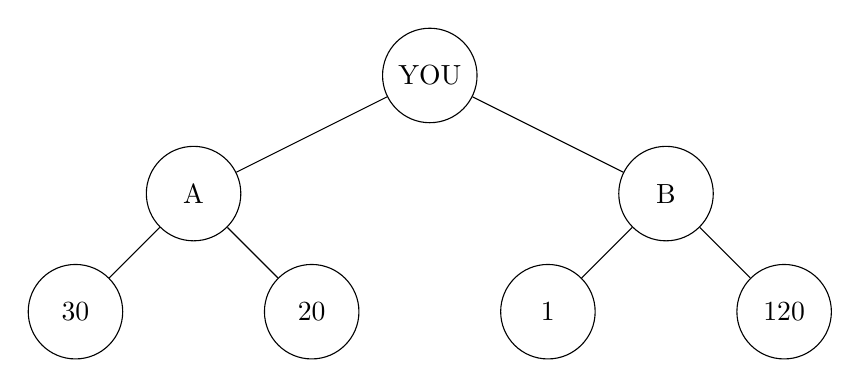
\begin{tikzpicture}[sibling distance=10em,
        every node/.style={circle, draw, minimum size=1.2cm},
        level/.style={sibling distance=6cm/#1}]

        \node (Root) {YOU}
        child {
            node {A}
            child { node {30} }
            child { node {20} }
        }
        child {
            node {B}
            child { node {1} }
            child { node {120} }
        };

    \end{tikzpicture}
    \captionof{figure}{Grafik zur Veranschaulichung des Gedankenexperimentes}
    \label{fig:thought-experiment}
\end{center}
\vspace{1em}

Ein solches Verfahren kann nun genutzt werden um unterschiedliche Spielz\"uge zu vergleichen und den Bestm\"oglichen - unter Ber\"ucksichtung der sp\"ateren Z\"uge des Gegners - auszuw\"ahlen.
Jedoch beinhaltet dieser Algorithmus einen Nachteil - es werden auch Spielz\"uge betrachtet, die nicht infrage kommen, da ein Spieler diesen Zug niemals w\"ahlen wird.

\subsubsection{Alpha-Beta-Pruning}\label{subsubsec:alpha-beta-pruning}
Dieses Problem kann mithilfe des Alpha-Beta-Prunings drastisch reduziert werden.
Hierbei werden Hilfsvariablen (alpha und beta) durchgereicht.
Diese Verbesserung muss Zugfolgen, die das Ergebnis unbeeinflusst lassen, nicht mehr kontrolliert.
Beim Gedankenexperiment muss somit nach dem Gegenstand im Wert von 1~\euro{} kein weiterer Knoten untersucht werden, da der Spieler YOU diesen Pfad (im Beispiel die Schublade B) nicht w\"ahlen wird.
Das liegt daran, dass f\"ur ihn die Schublade A wesentlich interessanter ist.
Selbstverst\"andlich nur unter Ber\"ucksichtigung, dass der Andere seinen Verlust minimieren m\"ochte.

\subsubsection{Vergleich der Algorithmen}\label{subsubsec:vergleich-der-algorithmen}
Um die Bedeutung dieser Variante zu verdeutlichen, folgt nun ein Vergleich beider Verfahren.
Dabei wird zuerst dieselbe Karte mit unterschiedlichen Suchbaumtiefen getestet.
Es treten in den Tiefen 3 bis 8 jeweils zwei Spieler gegeneinander an\footnote{Die Suchbaumtiefe 8 wurde auf einem Labor-PC der OTH Regensburg durchgef\"uhrt. N\"ahere Informationen siehe Kapitel~\ref{subsec:technische-daten}}.
Es wird je einmal der erste Spieler und einmal der zweite Spieler mit Alpha-Beta gestartet.

\vspace{1em}
\begin{minipage}{\linewidth}
    \centering
    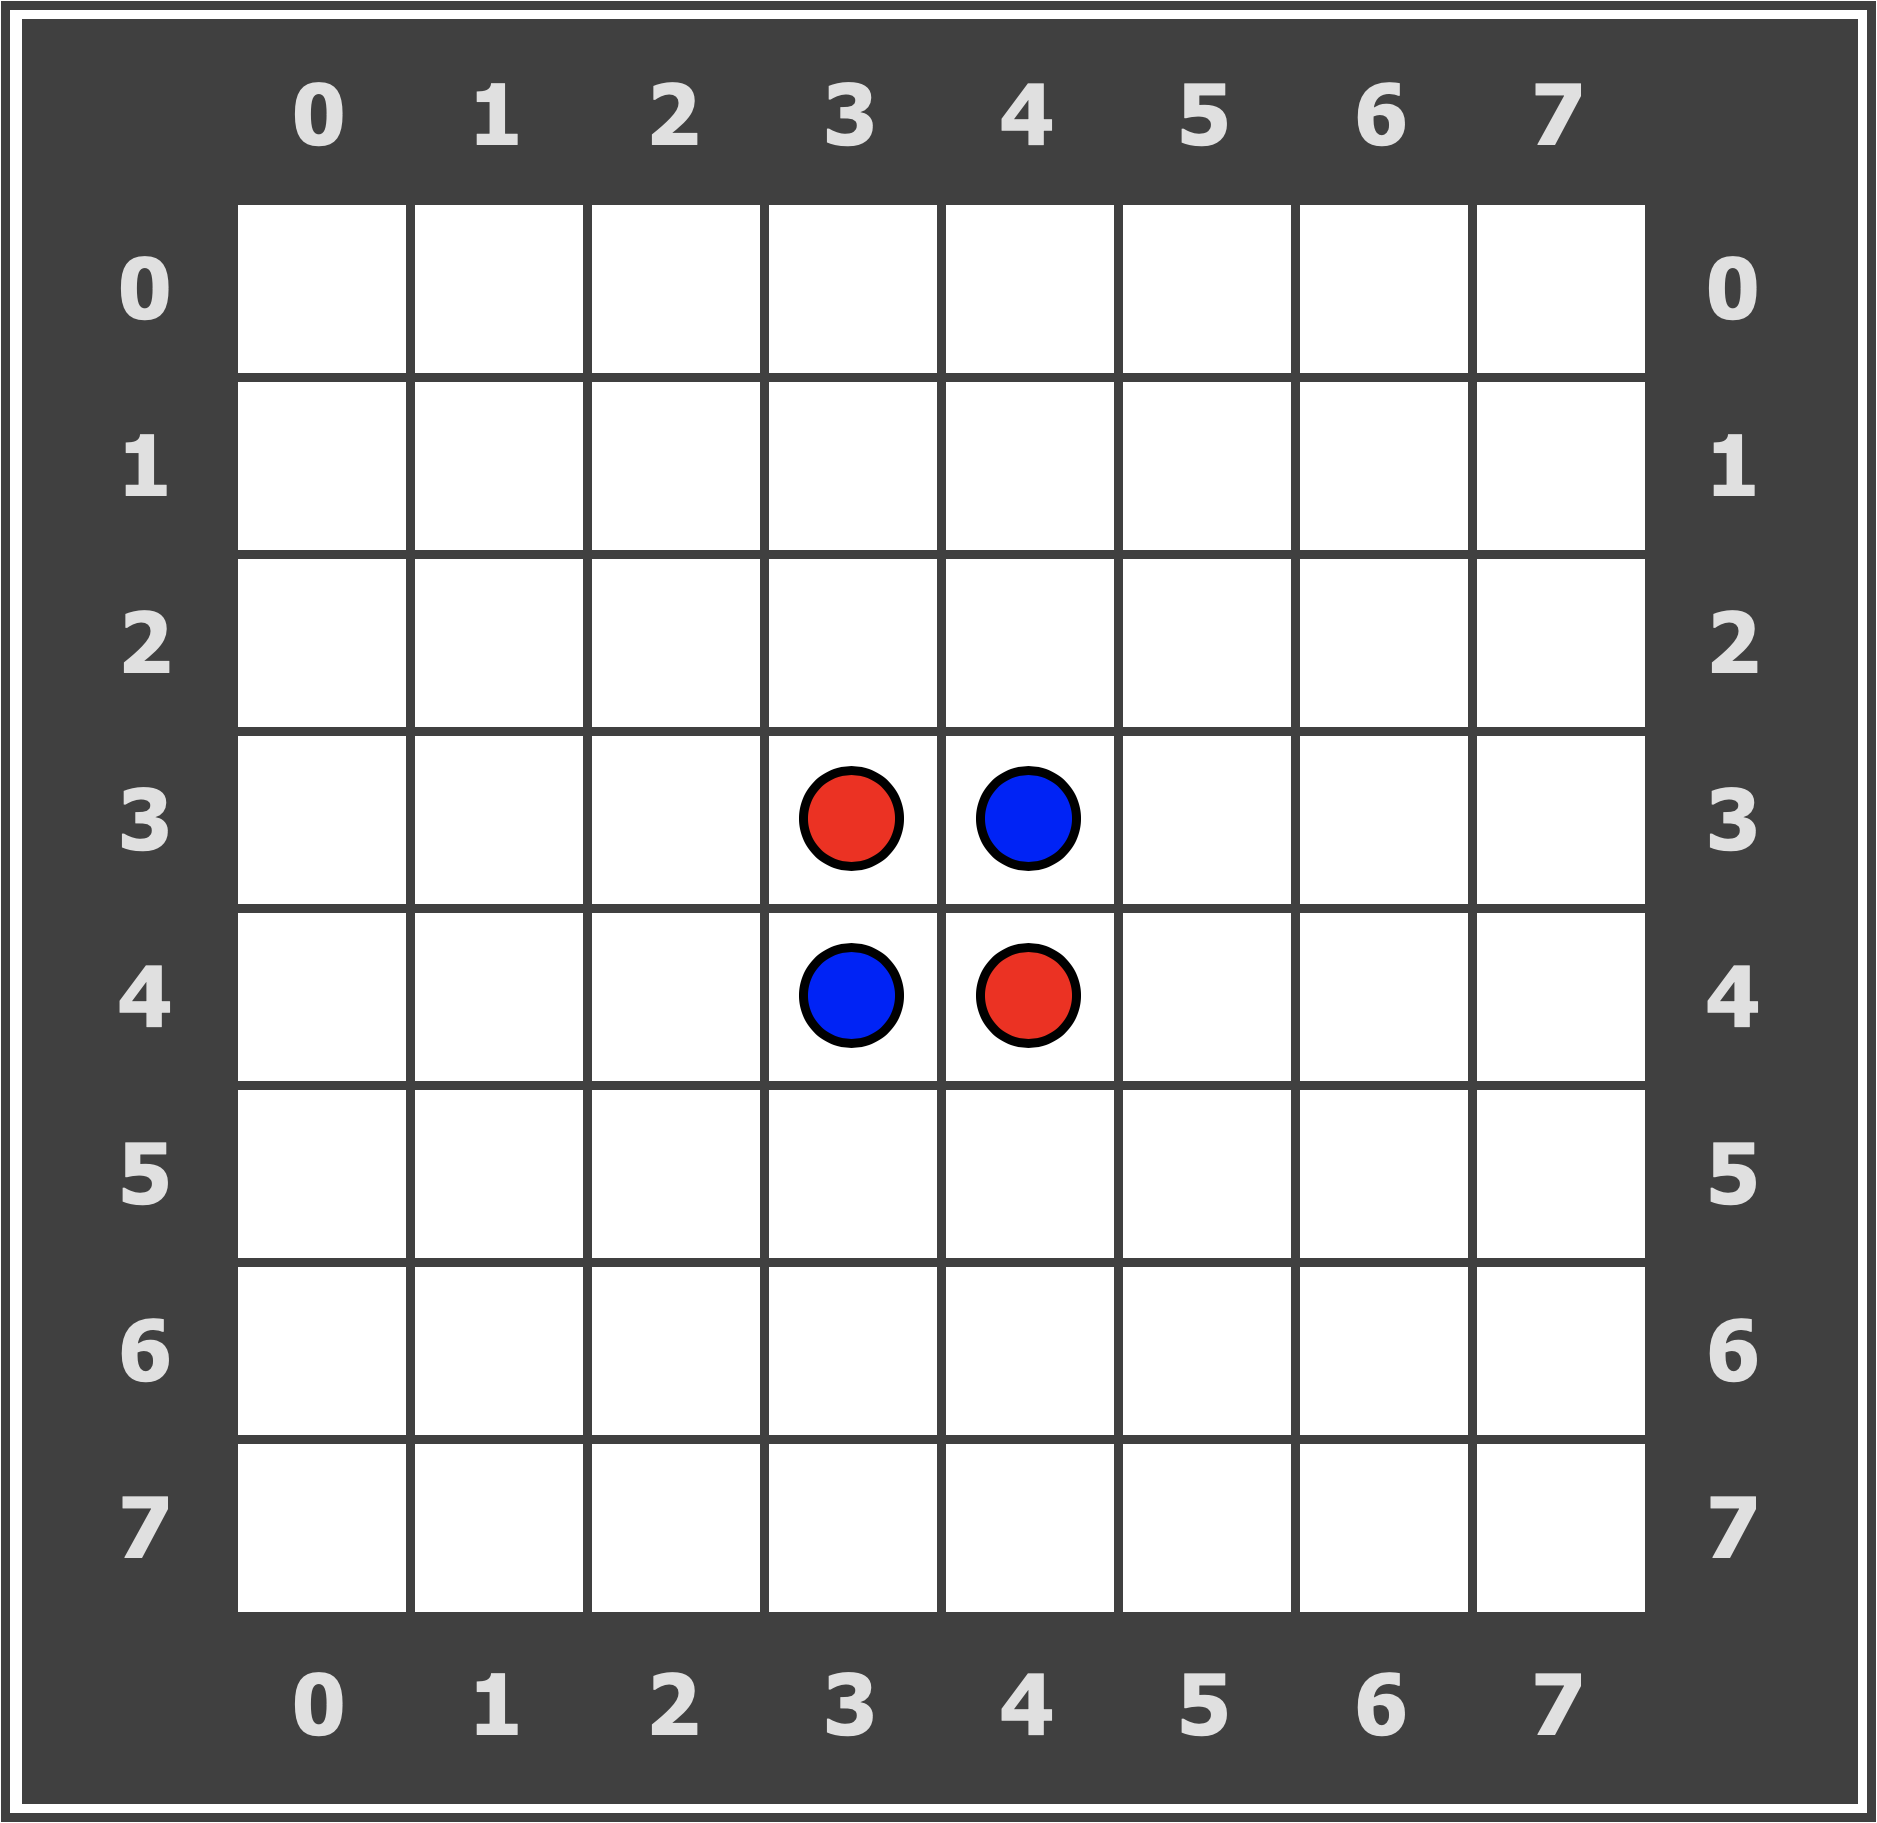
\includegraphics[width=0.3\linewidth]{pics/statistic-map}
    \captionof{figure}[Karte f\"ur Statisitk]{Verwendete Karte f\"ur den Vergleich von Minimax und Alpha-Beta}
    \label{fig:statistic-map}
\end{minipage}
\vspace{1em}

Es wird aus folgenden Gr\"unden die Karte aus Abbildung~\ref{fig:statistic-map} zu Beginn gew\"ahlt:
\begin{enumerate}
    \item Es gibt nur zwei Spieler, womit beide Verfahren gegeneinander antreten k\"onnen.
    \item Es gibt keine Spezialsteine, was das Spiel einfacher gestaltet und beim Vergleich der Algorithmen vorerst nicht von Bedeutung ist.
    \item Die verwendete Karte ist komplett symmetrisch, wodurch eine Fairness f\"ur beide Spieler garantiert wird.
    \item Es handelt sich um eine relativ kleine Karte, damit die Berechnungen zeitlich einigerma"sen eingegrenzt werden k\"onnen.
\end{enumerate}

\vspace{1em}
\begin{minipage}{\linewidth}
    \centering
    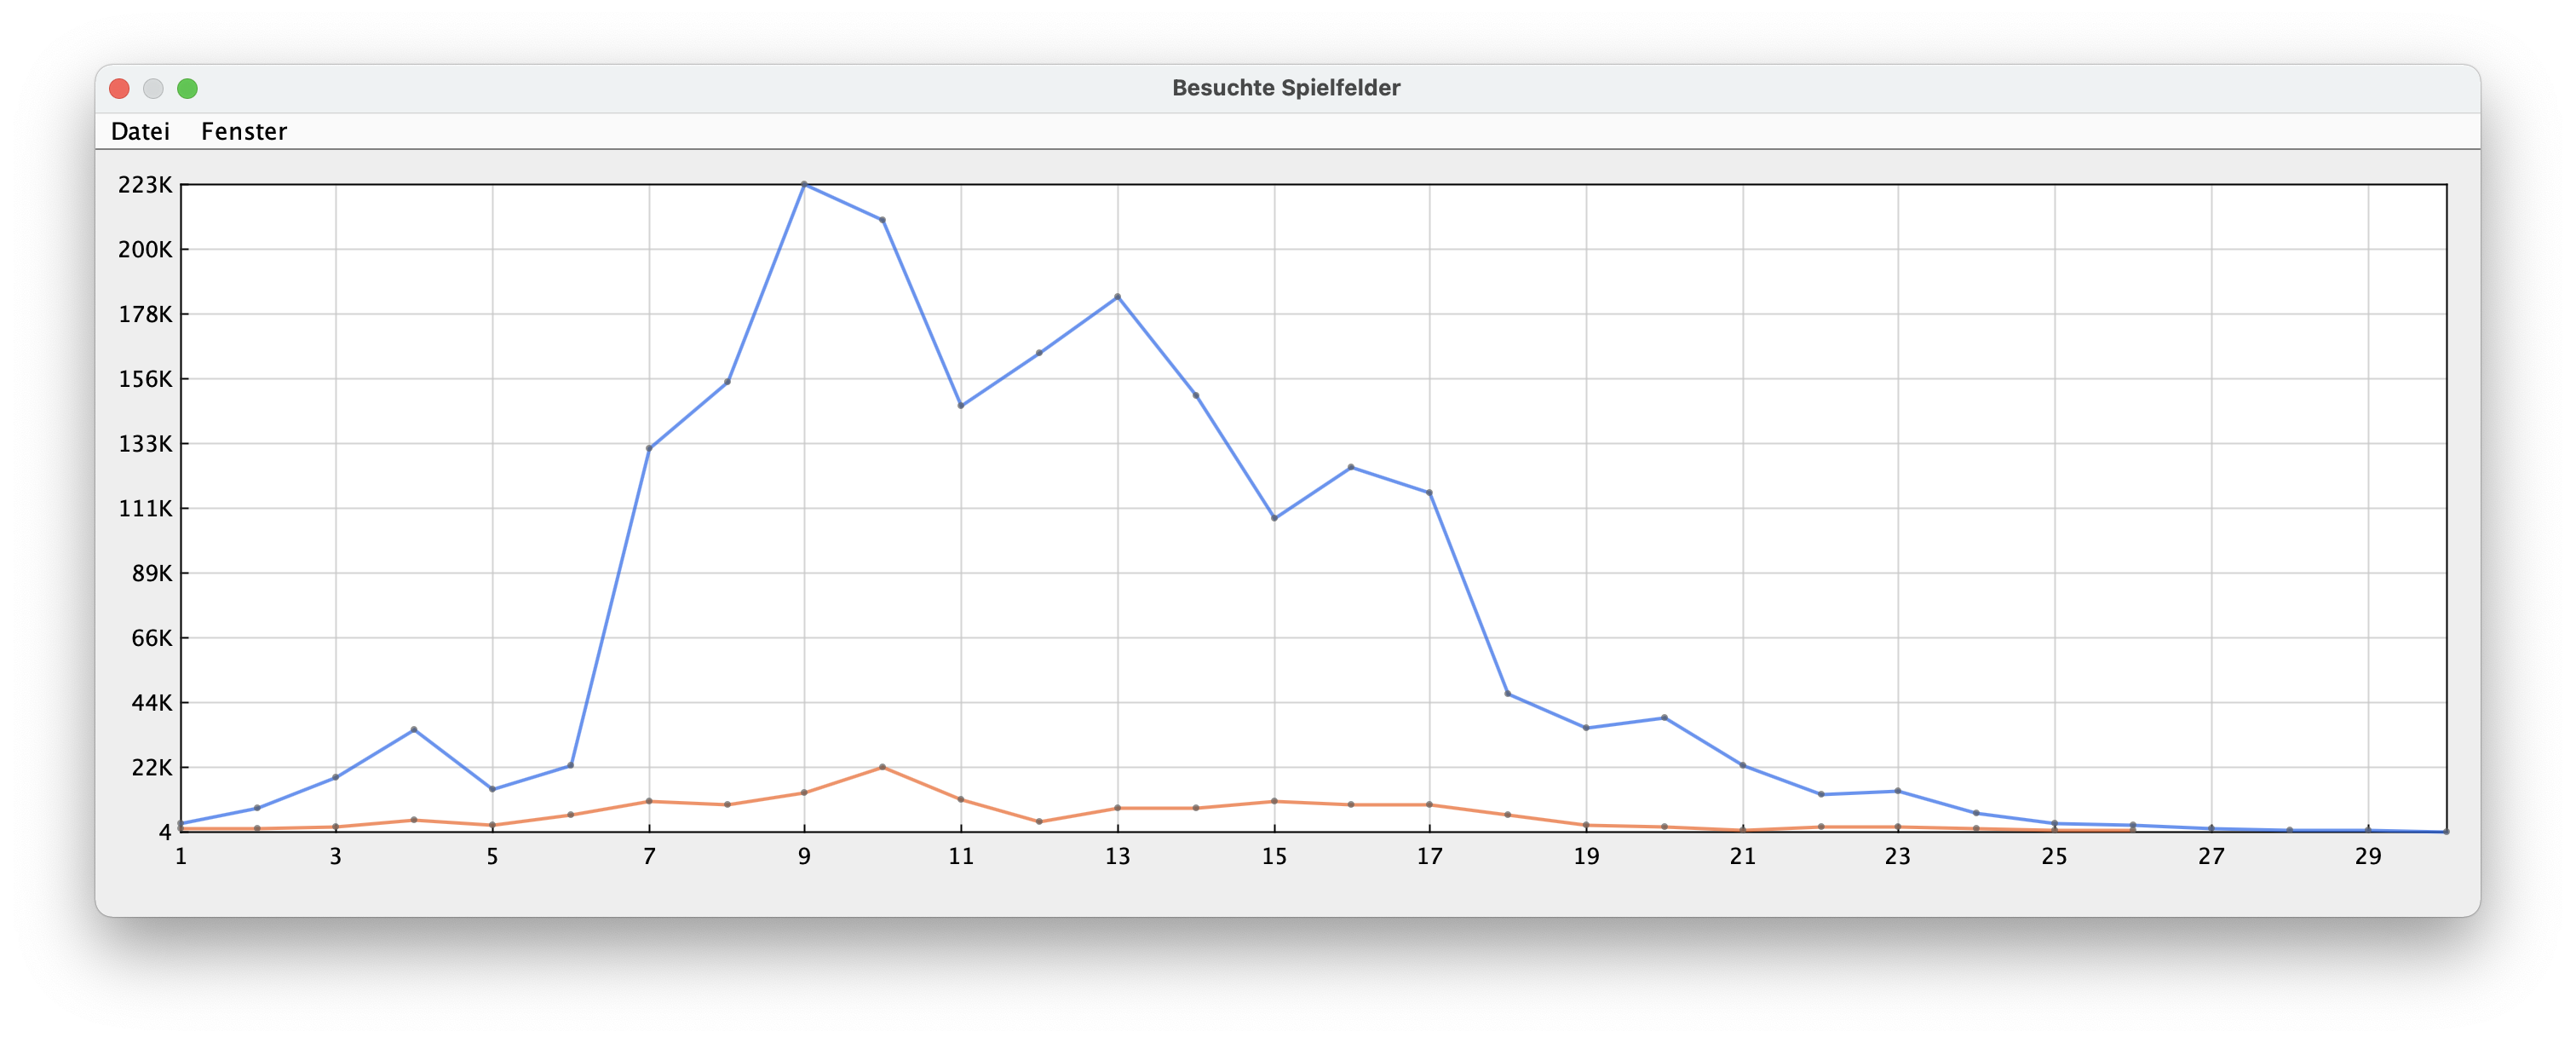
\includegraphics[width=0.9\linewidth]{statistic/ORIGINAL-D5-01/ST-01-D5-LD}
    \captionof{figure}[Statistik f\"ur Tiefe 5]{Diese Statistik wurde bei einem Spiel der Tiefe 5 aufgenommen.}
    \label{fig:statistic-screen}
\end{minipage}
\vspace{1em}

In Abbildung~\ref{fig:statistic-screen} sind sowohl \"uberpr\"ufte Karten ohne Alpha-Beta (blaue Linie), als auch mit Alpha-Beta (orange Linie) zu sehen.
Hierbei ist klar ersichtlich, dass Alpha-Beta-Pruning einen enormen Leistungsvorteil liefert.
Der obige Screenshot stammt aus der selbstentwickelten Software GameAnalyzer.
Mehr dazu in Kapitel~\ref{sec:spielanalyse}.

Die Tabelle~\ref{tab:search-depth} liefert eine \"Ubersicht \"uber alle getesteten Suchbaumtiefen dieser Karte.

\vspace{1em}
\begin{table}[!h]
    \centering
    \begin{tabular}{|l|c|c|}
        \hline
        \textbf{Tiefe} & \textbf{Alpha-Beta} & \textbf{Minimax}\\
        \hline
        3 & 1.079,5 & 2.434,5\\
        \hline
        4 & 5.985,5 & 18.417,5\\
        \hline
        5 & 22.653 & 244.854,5\\
        \hline
        6 & 133.657,5 & 1.313.347\\
        \hline
        7 & 419.537 & 28.802.230\\
        \hline
        8 & 1.898.497 & 449.424.275\\
        \hline
    \end{tabular}
    \caption{Besuchte Karten mit den Suchalgorithmen (Ergebnisse wurden gegl\"attet)}
    \label{tab:search-depth}
\end{table}
\vspace{1em}

Auf den ersten Blick wirken diese Zahlen nun ziemlich bedeutungslos.
Werden Sie jedoch in ein Koordinatensystem (siehe Abbildung~\ref{fig:statistic-graph}) eingetragen und eine Linie eingezeichnet, kann man den Verlauf bei weiteren Suchbaumtiefen beider Algorithmen erahnen.

\vspace{1em}
\begin{minipage}{\linewidth}
    \centering
    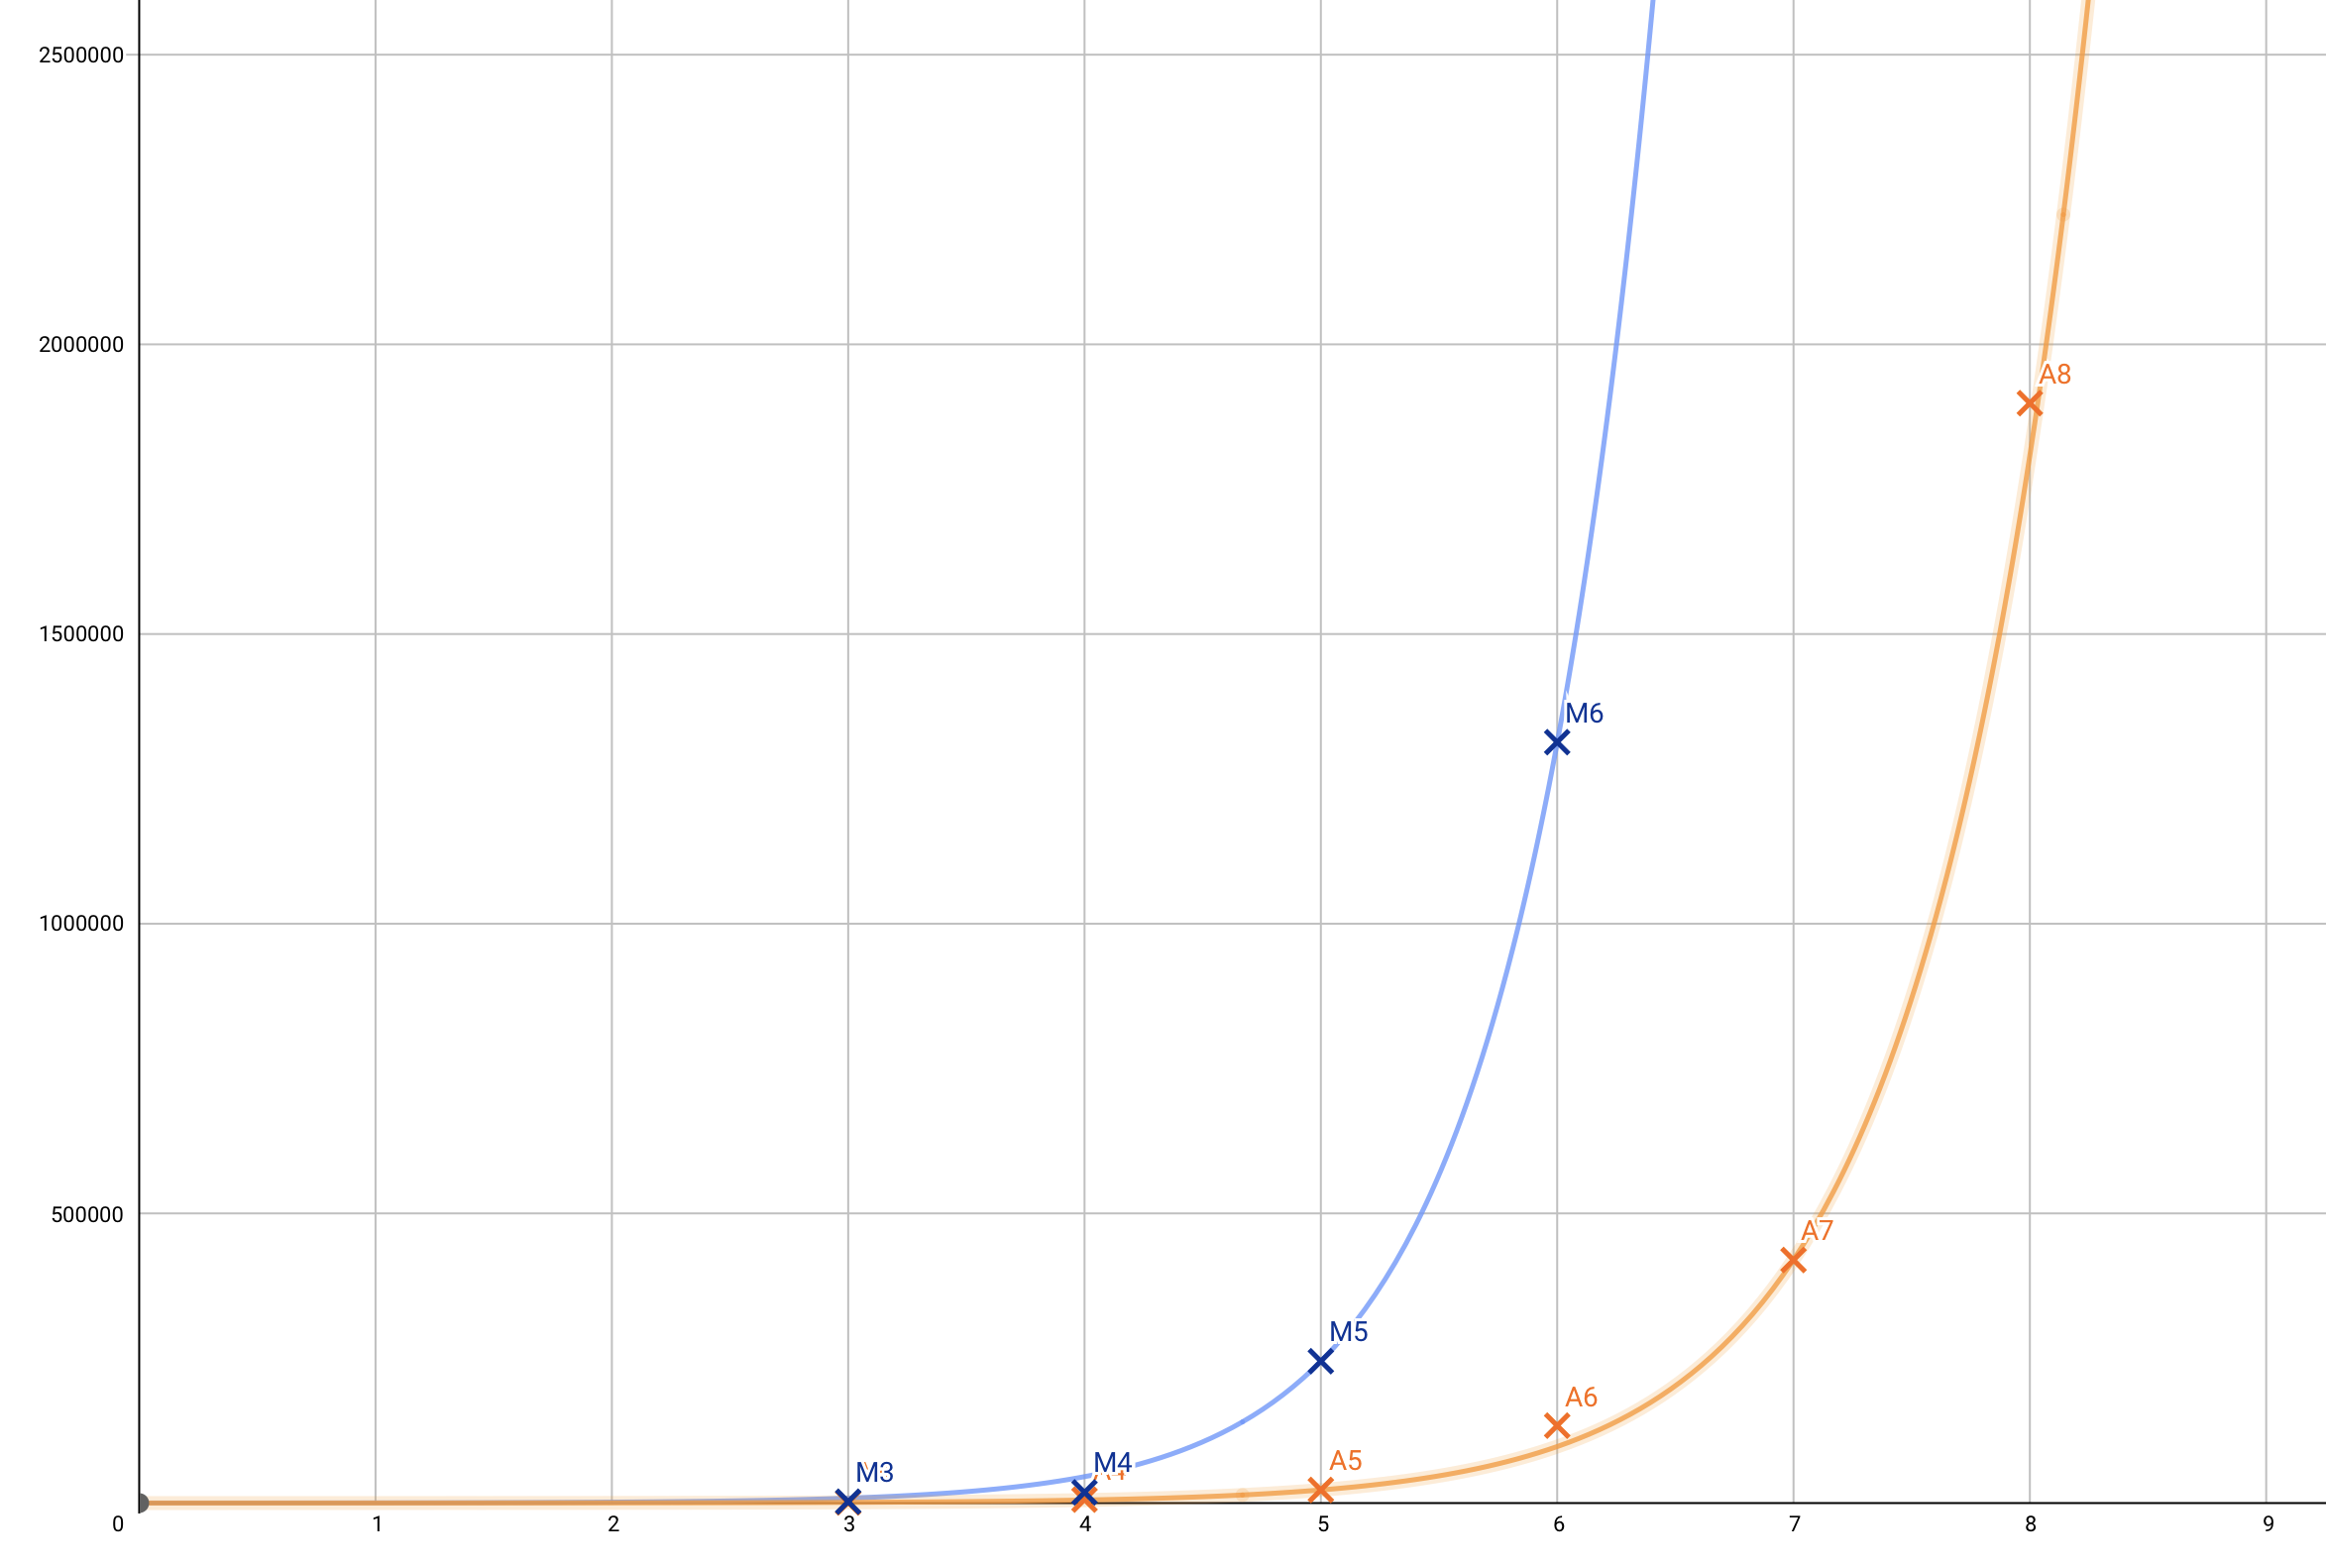
\includegraphics[width=0.7\linewidth]{pics/statistic-graph}
    \captionof{figure}[Suchbaumtiefen in Koordinaten]{Suchbaumtiefen in ein Koordinatensystem eingetragen}
    \label{fig:statistic-graph}
\end{minipage}
\vspace{1em}

Der Aufwand, alle m\"oglichen Spielzust\"ande zu vergleichen, w\"achst bei beiden Verfahren exponentiell mit der Anzahl der Suchbaumtiefe.
Jedoch bewirkt das Alpha-Beta-Pruning eine gestauchtere Kurve als der Minimax-Algorithmus ohne Alpha-Beta-Pruning.

Bei gleicher Anzahl an bewerteten Feldern wird mit Alpha-Beta-Pruning der Suchbaum tiefer analysiert und dadurch mehr Z\"uge miteinander verglichen.
Das f\"uhrt dazu, dass bei gleichem Zeitaufwand (\corresponds gleiche Anzahl an analysierten Spielzust\"anden) das beste Ergebnis einer \underline{tieferen} Suchbaumebene gefunden wird.

\newpage

Um diese Aussage adequate zu best\"atigen sind vier weitere Karten (siehe Abbildung~\ref{fig:additional-statistic-maps}) aufgef\"uhrt, bei denen erneut Tests durchgef\"uhrt werden.
Die Statistiken zum Vergleich der Algorithmen befindet sich jeweils unterhalb der textuellen Vorstellung der einzelnen Karten.
Die blaue Linie stellt hierbei immer den Minimax-Algorithmus und die orange Linie das Alpha-Beta-Pruning dar.

\textbf{Reversi Cuboid:}
Diese Map basiert auf dem Grundspiel von Reversi, jedoch sind hier vier Bereiche angeordnet.
Durch diese Anordnung ist diese Map fair und es gibt einige Spezialfelder, die jedoch erst im sp\"ateren Verlauf des Spieles erreichbar sind.
Durch diese Karte soll getestet werden wie sich 8-Spieler-Karten auf die beiden Algorithmen auswirkt.
Diese Karte wird aufgrund vieler Spieler auf Tiefe 4 durchlaufen.
Dabei wird als erster und zweiter Spieler der Client zum Testen der Algorithmen verwendet.
Die anderen Spieler verwenden den triviale Client, welcher zu Beginn des Semesters jedem Team ausgeh\"andigt wird.

\begin{minipage}{\linewidth}
    \centering
    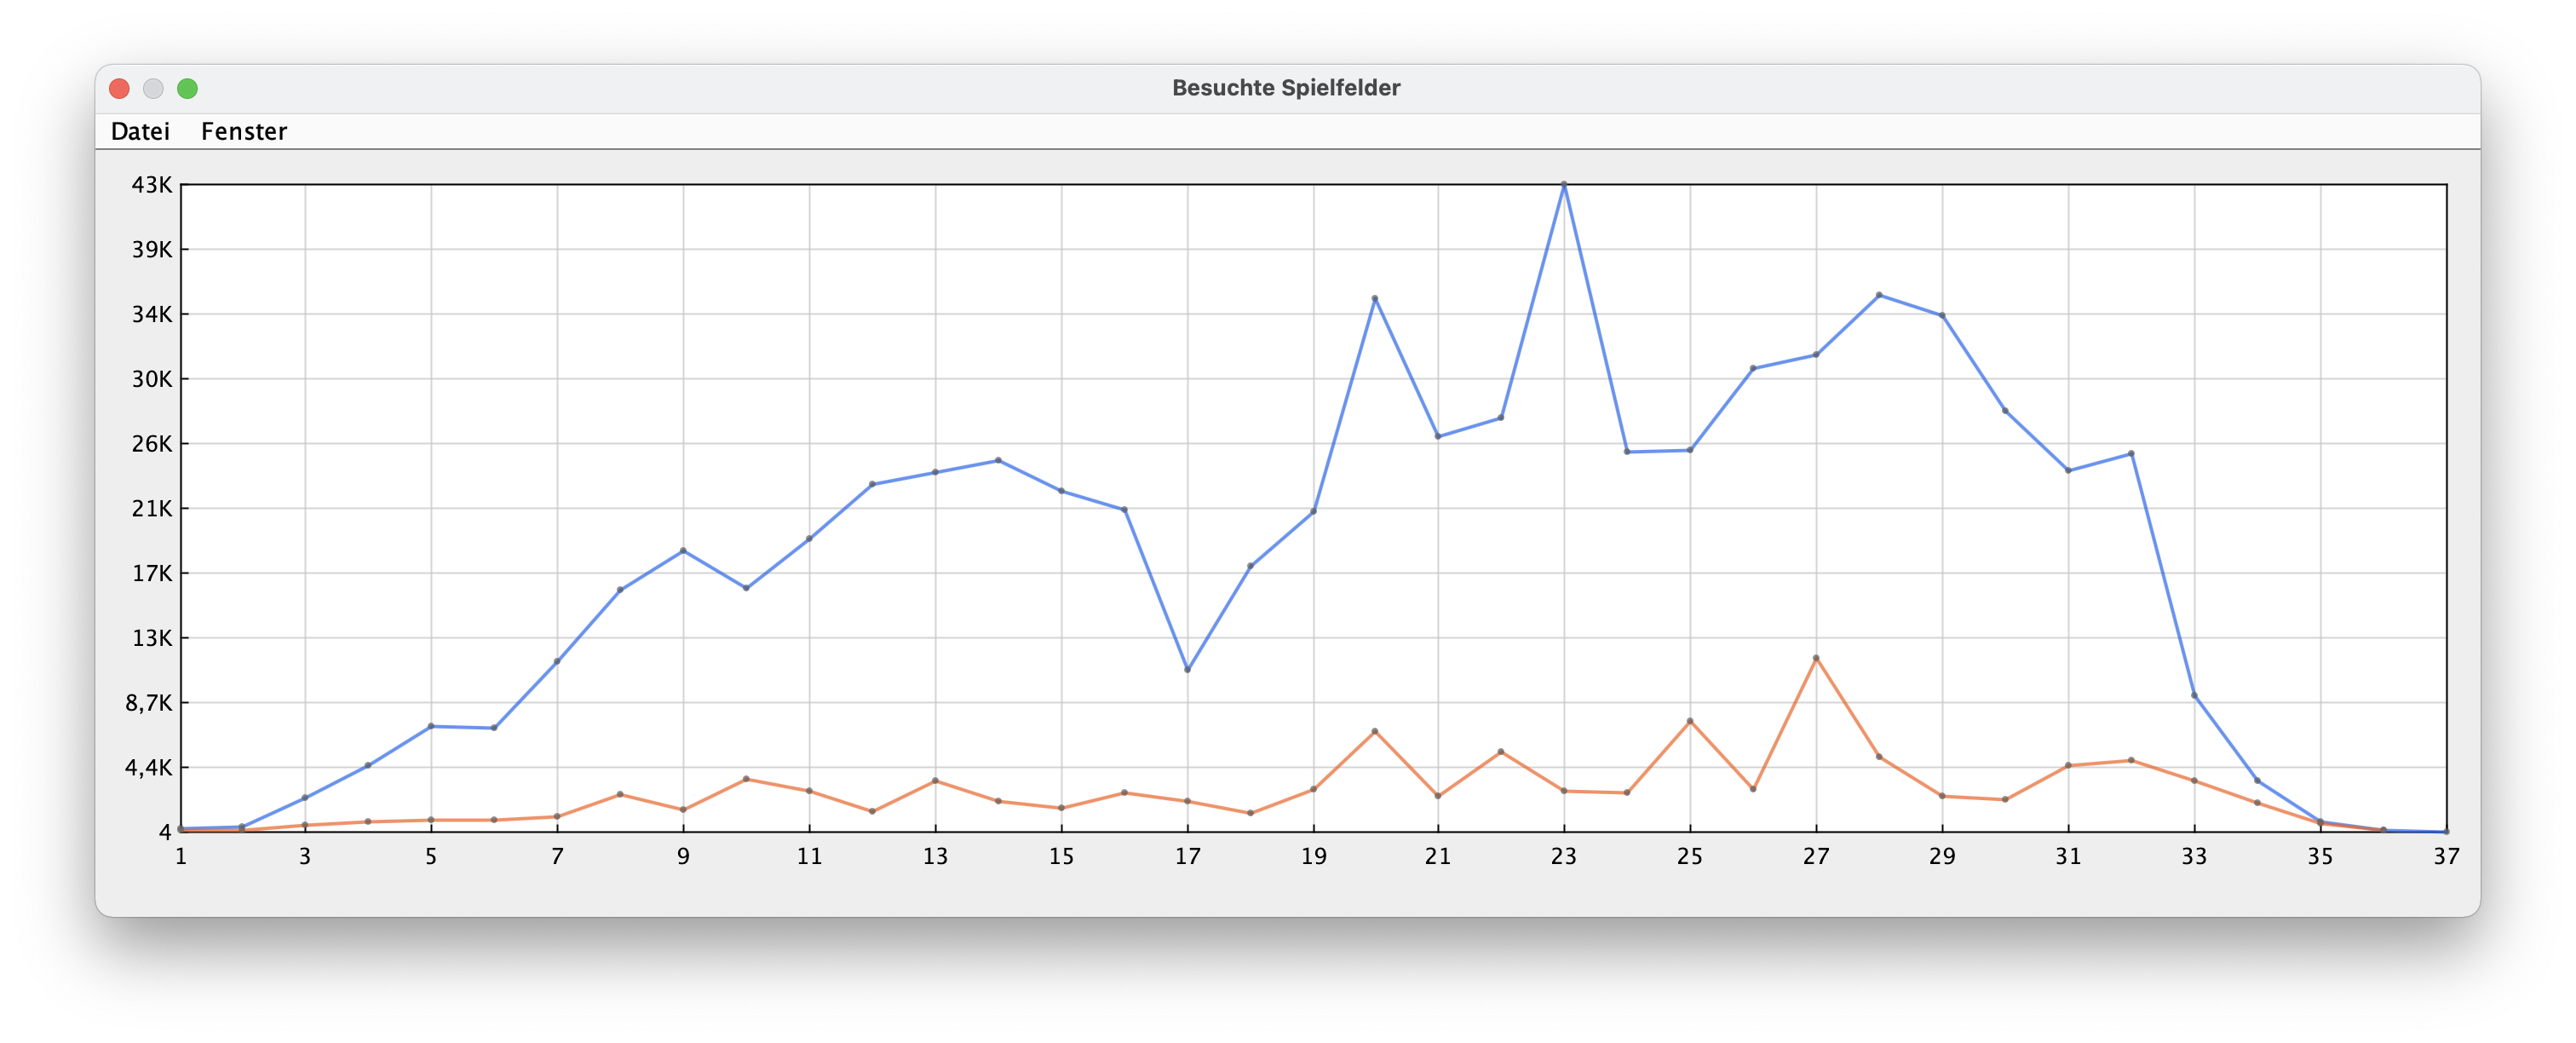
\includegraphics[width=0.9\linewidth]{statistic/CUBOID-01/ST-01-D4-LD}
    \captionof{figure}{Vergleich der Algorithmen auf der Karte Reversi Cuboid}
    \label{fig:statistic-graph-cuboid}
\end{minipage}
\vspace{1em}

\textbf{Cupcake:}
Diese Map hat bereits zu Beginn sehr viele unterschiedliche Startpositionen.
Was dazu f\"uhrt, dass der Suchbaum bereits zu Beginn sehr breit ist und somit sehr stark anw\"achst.
Er beeinhaltet jedoch keine Transitionen oder Sonstige Spezialfelder, wodurch die Anzahl damit jedoch zu einem gewissen Teil eingeschr\"ankt werden.
Die Karte wird auf Tiefe 4 durchlaufen.

\begin{minipage}{\linewidth}
    \centering
    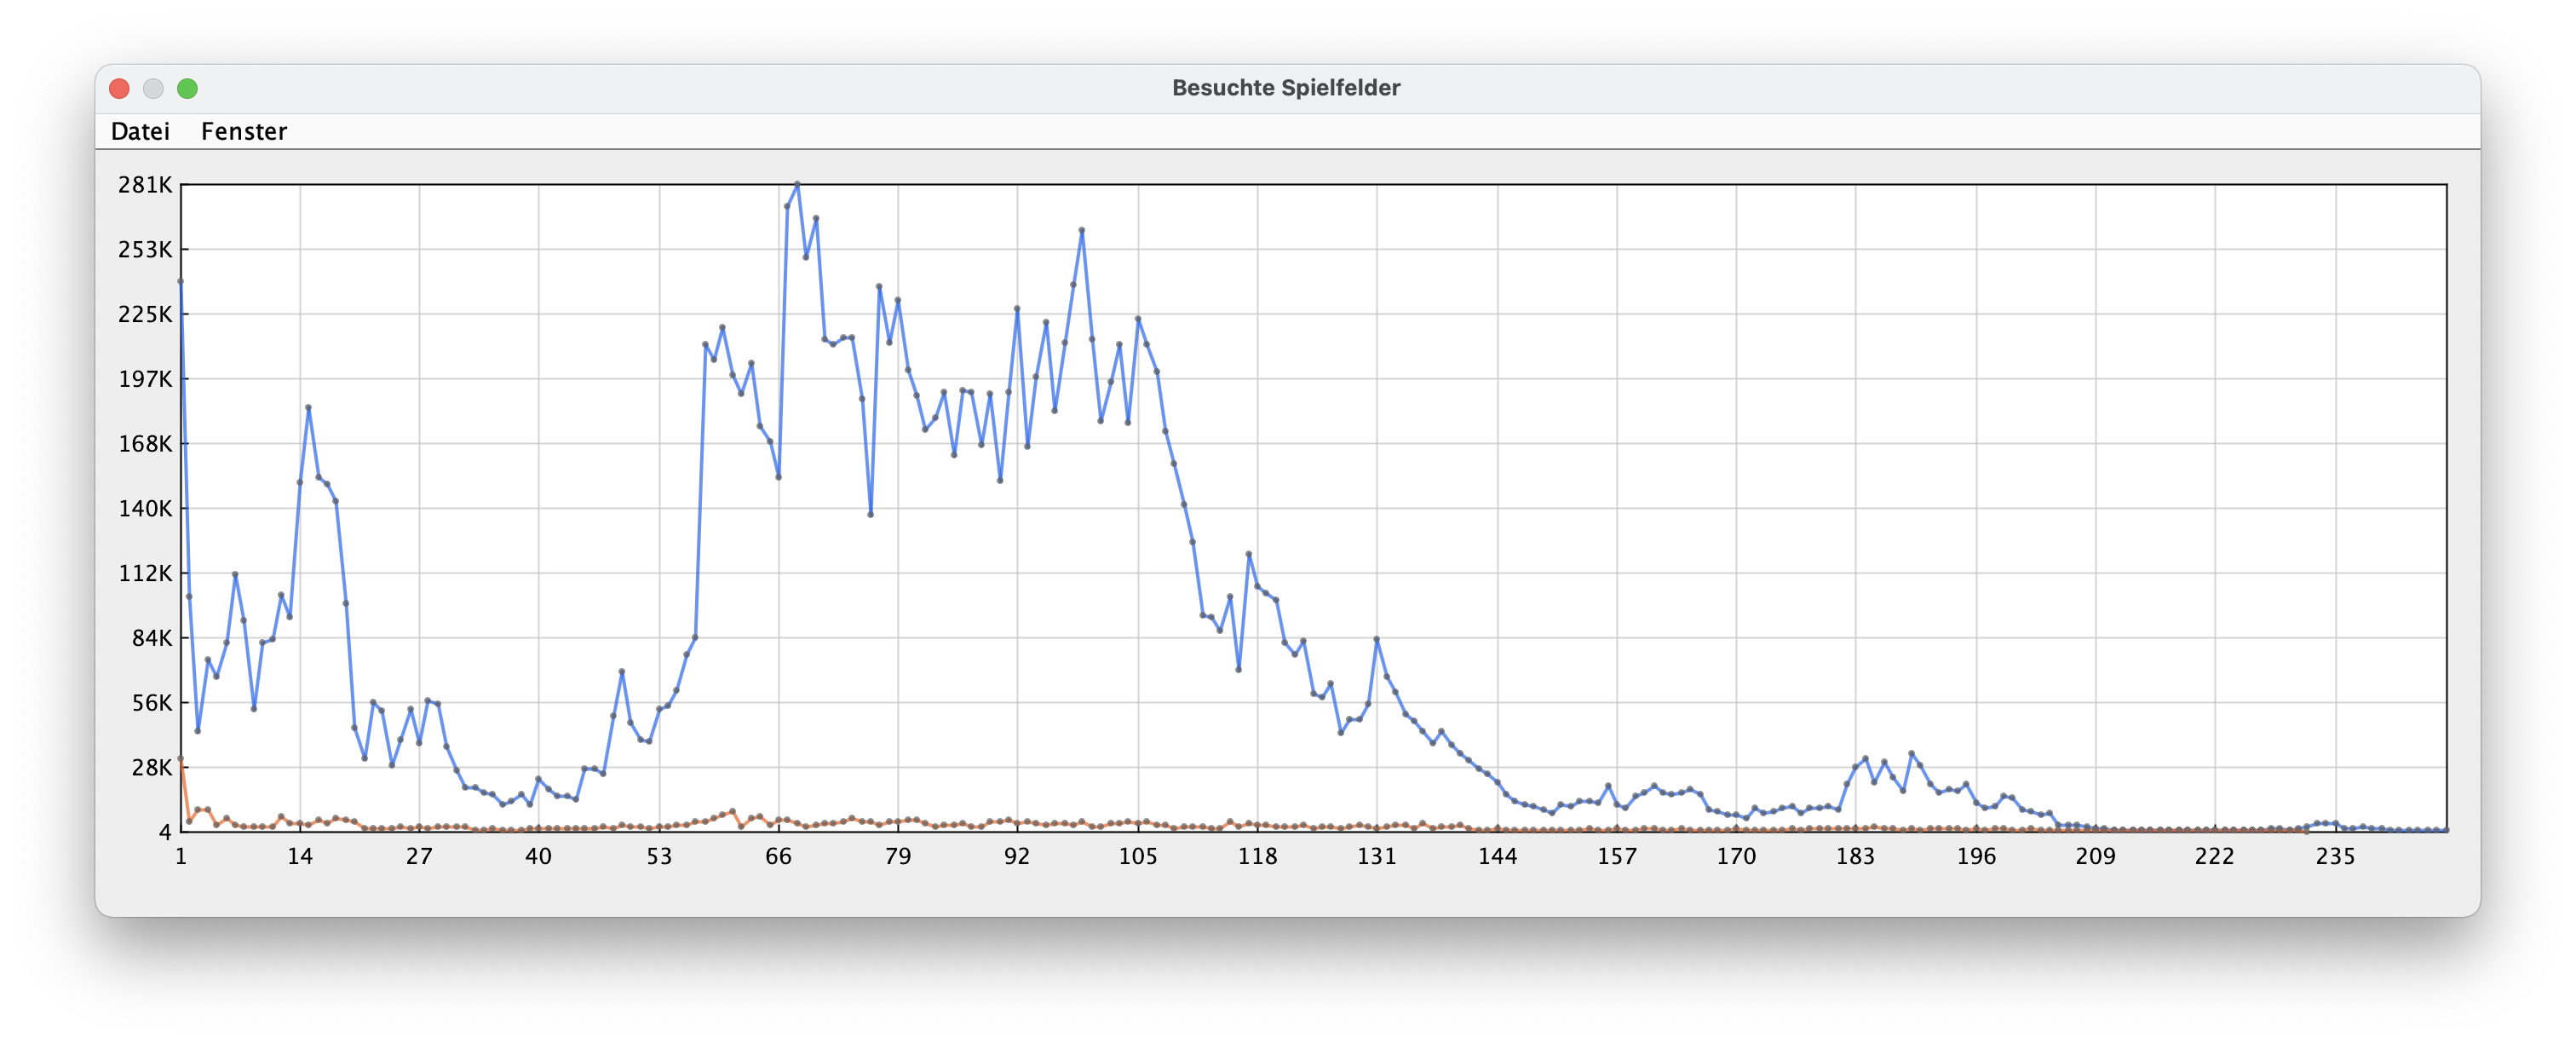
\includegraphics[width=0.9\linewidth]{statistic/CUP-01/ST-01-D4-LD}
    \captionof{figure}{Vergleich der Algorithmen auf der Karte Cupcake}
    \label{fig:statistic-graph-cupcake}
\end{minipage}
\vspace{1em}

\textbf{Dog Extended:}
Bei der Dog Extended Karte handelt es sich um die Karte, die f\"ur alle Abgaben w\"ahrend dem Semester verwendet wird.
Aus diesem Grund wird auch die Map Dog Extended bei diesem Test \"uberpr\"uft.
In dieser Karte sind Transitionen sowie alle m\"oglichen Spezialsteine integriert um alle Abh\"anigkeiten zu testen.
Diese Karte wird auf Tiefe 5 durchlaufen.

\begin{minipage}{\linewidth}
    \centering
    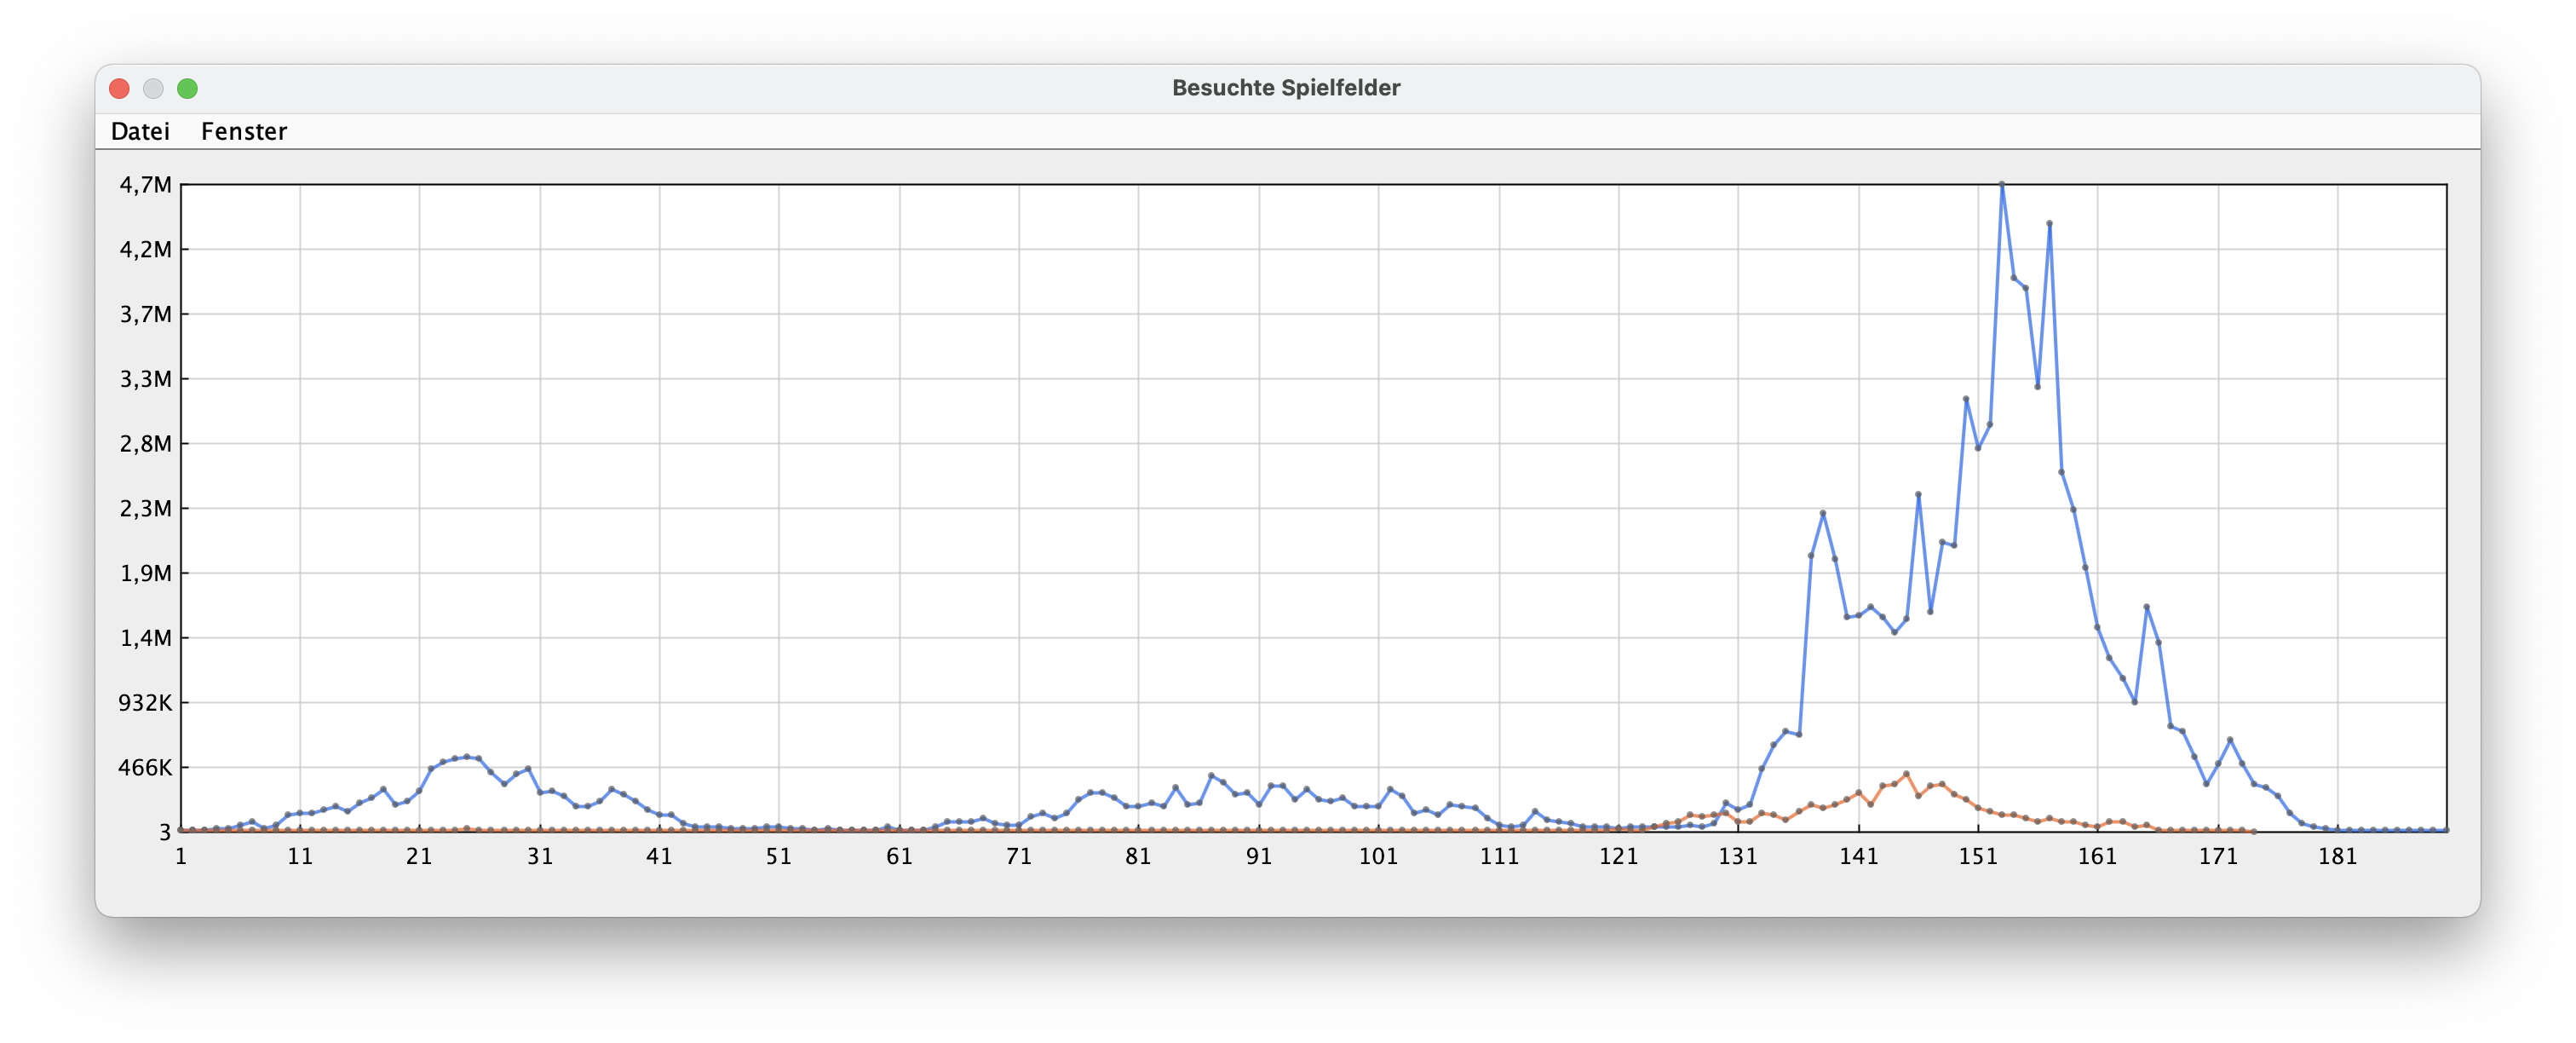
\includegraphics[width=0.9\linewidth]{statistic/DOG-02/ST-01-D4-LD}
    \captionof{figure}{Vergleich der Algorithmen auf der Karte Dog Extended}
    \label{fig:statistic-graph-dog}
\end{minipage}
\vspace{1em}

\textbf{Europa:}
Die Europa Karte ist eine sehr gro\"se Map bei der jedoch viele Stellen aus L\"ochern bestehen und es zudem eine Menge an Kanten und Ecken gibt.
Dadurch wird die Spielfeldgewichtung unter Probe gestellt um zu testen ob es hierbei zu starken Abweichungen kommt, da die Gewichtung hier oft gleiche Ergebnise liefern k\"onnte und somit wenig weggek\"urzt werden kann.
Diese Karte wird auf Tiefe 3 durchlaufen, da es eine sehr gro"se Karte mit drei Spielern ist.
Dabei wird als erster Spieler der triviale Client verwendet.

\begin{minipage}{\linewidth}
    \centering
    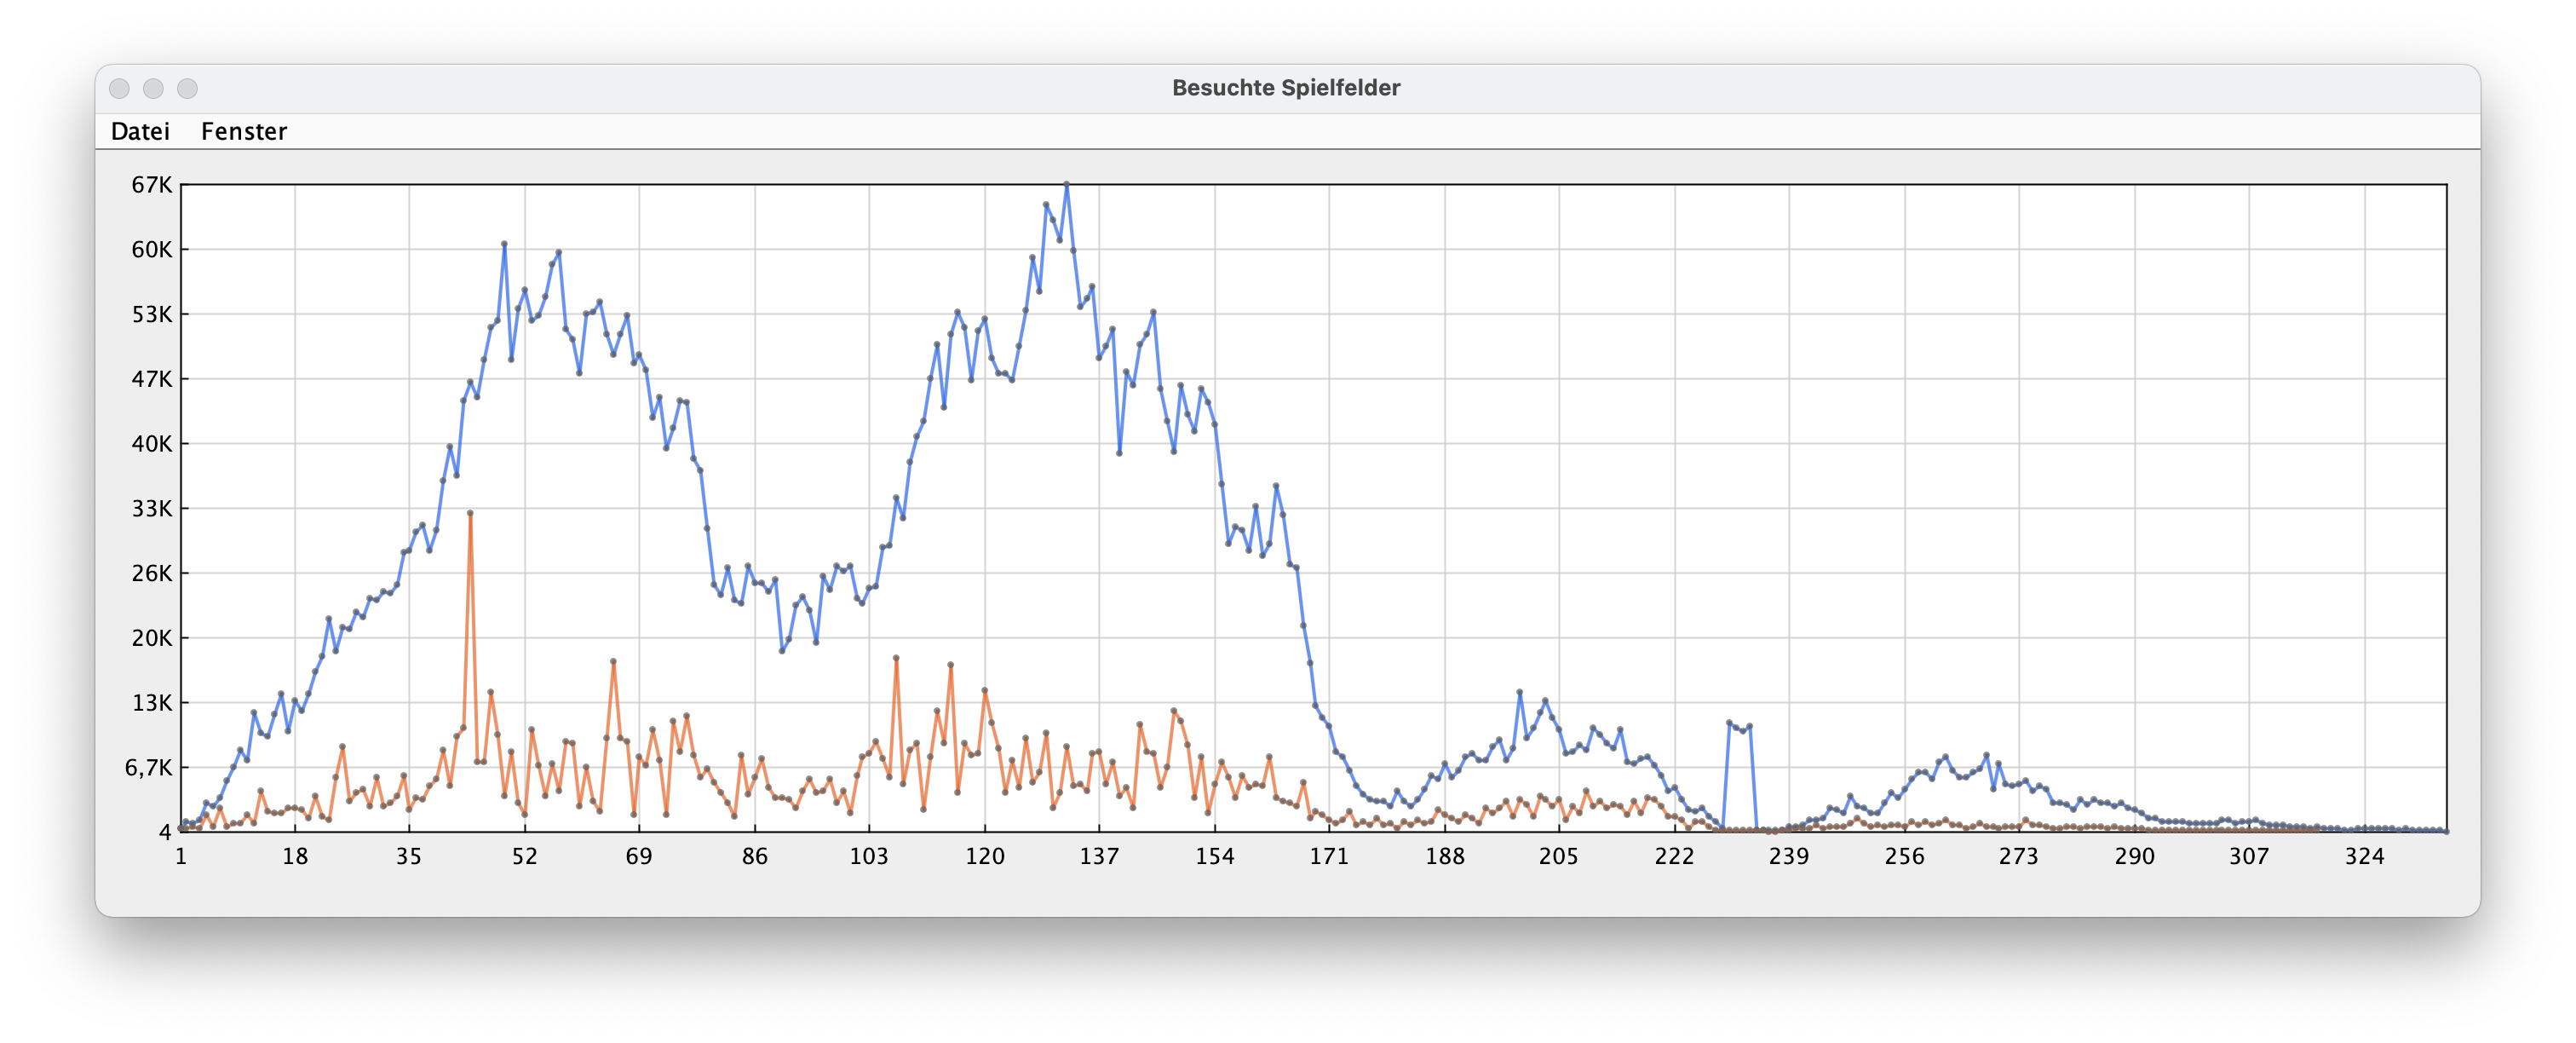
\includegraphics[width=0.9\linewidth]{statistic/EUROPA-02/ST-01-D3-LD}
    \captionof{figure}{Vergleich der Algorithmen auf der Karte Europa}
    \label{fig:statistic-graph-europa}
\end{minipage}
\vspace{1em}

\vspace{1em}
\begin{table}[!h]
    \centering
    \begin{tabular}{|l|c|c|c|}
        \hline
        \textbf{Karte} & \textbf{Tiefe} & \textbf{Alpha-Beta} & \textbf{Minimax}\\
        \hline
        Cupcake & 4 & 30.142 & 281.694\\
        \hline
        Reversi Cuboid & 6 & 11.459 & 48.656\\
        \hline
        Dog Extended & 5 & 978.310,5 & 4.357.785\\
        \hline
        Europa & 3 & 34.365 & 64.316,5\\
        \hline
    \end{tabular}
    \caption{Tabellarischer Vergleich der aufgef\"uhrten Statistiken (Ergebnisse wurden gegl\"attet)}
    \label{tab:additional-search-depth}
\end{table}
\vspace{1em}

Betrachtet man nun alle aufgef\"uhrten Karten kann man zwar jeweils einen Unterschied in der G\"ute des Alpha-Beta Prunings feststellen, jedoch wird hier klar ersichtlich, dass sich bei jeder getesteten Karte ein gewisser Leistungsvorteil ergibt.
Das Team hat sich genau aus diesen Gr\"unden dazu entschieden, auf jeder Karte standardm\"a"sig Alpha-Beta Purning zu aktivieren.

\vspace{1em}
\begin{figure}
    \centering
    \subfloat[Karte: Reversi Cuboid]{ 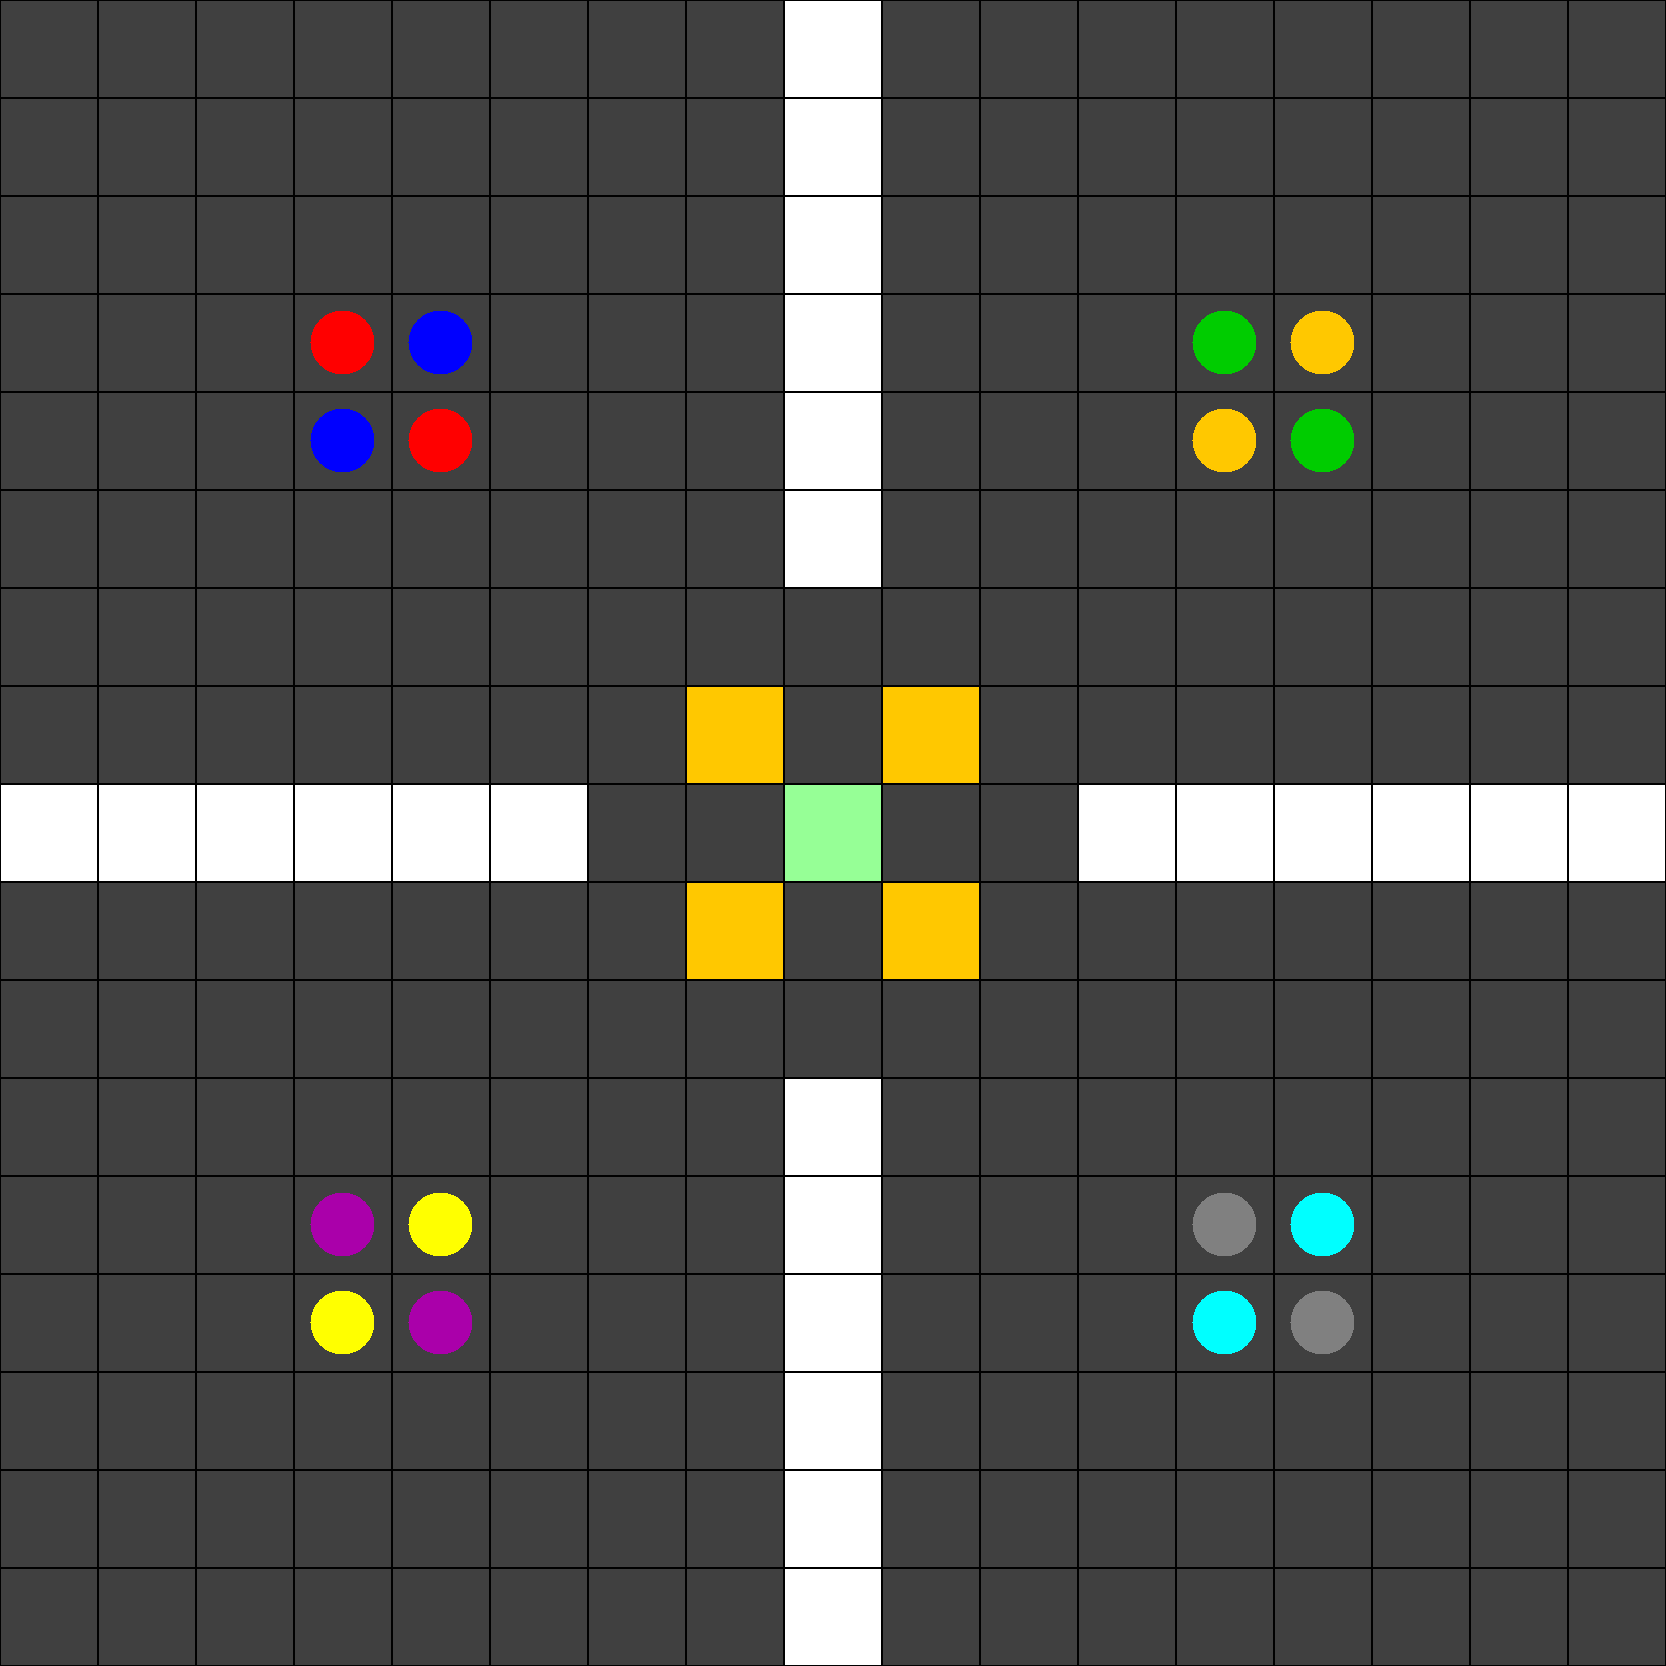
\includegraphics[width=0.5\linewidth]{pics/maps/reversi-cuboid} }
    \qquad
    \subfloat[Karte: Cupcake]{ 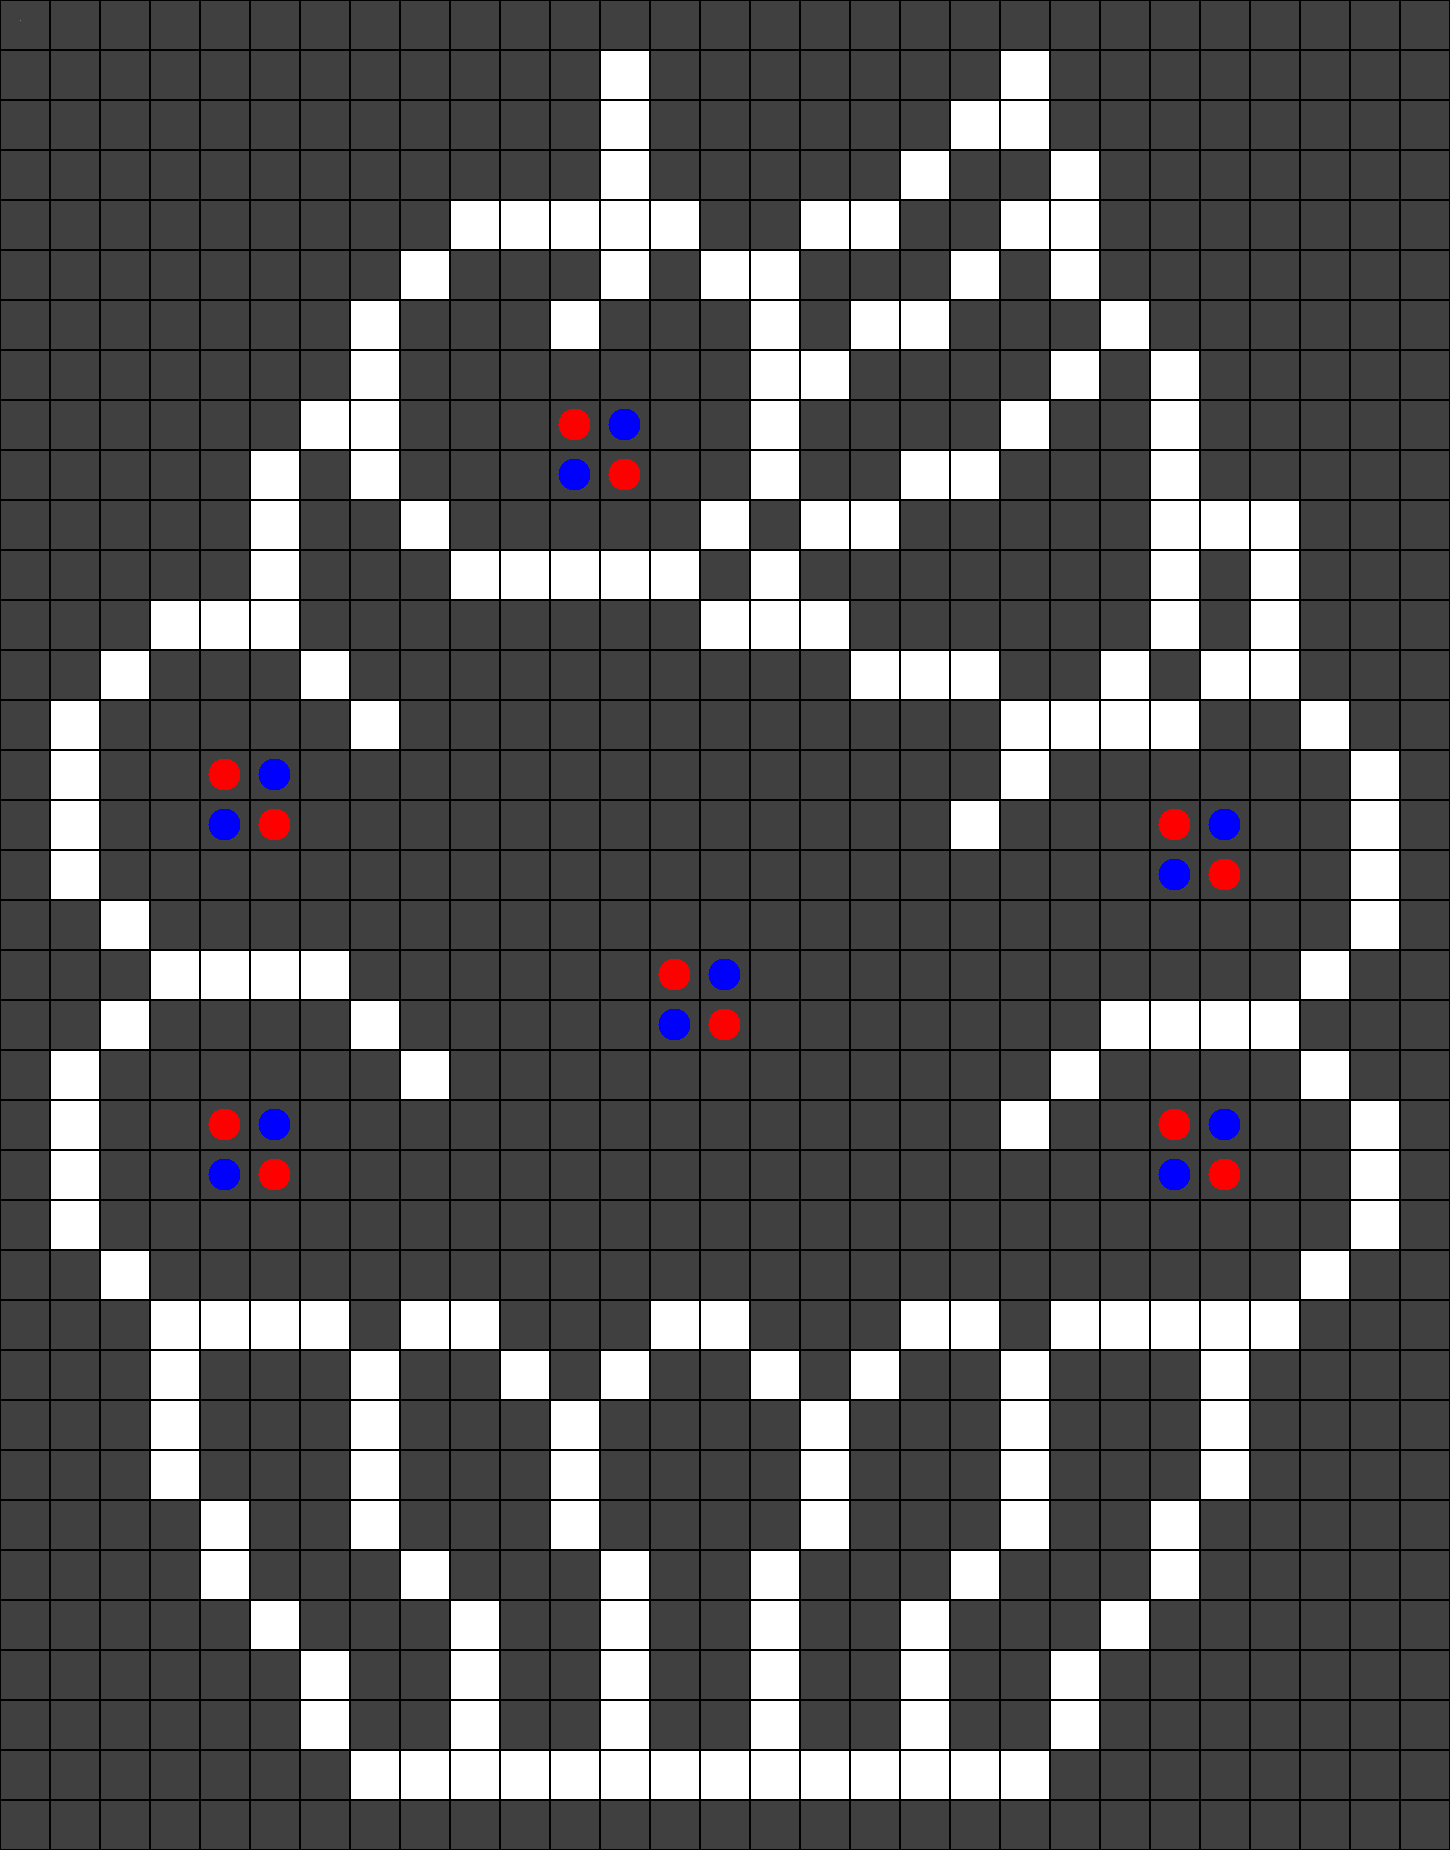
\includegraphics[width=0.4\linewidth]{pics/maps/cupcake} }
    \qquad
    \subfloat[Karte: Dog Extended]{ 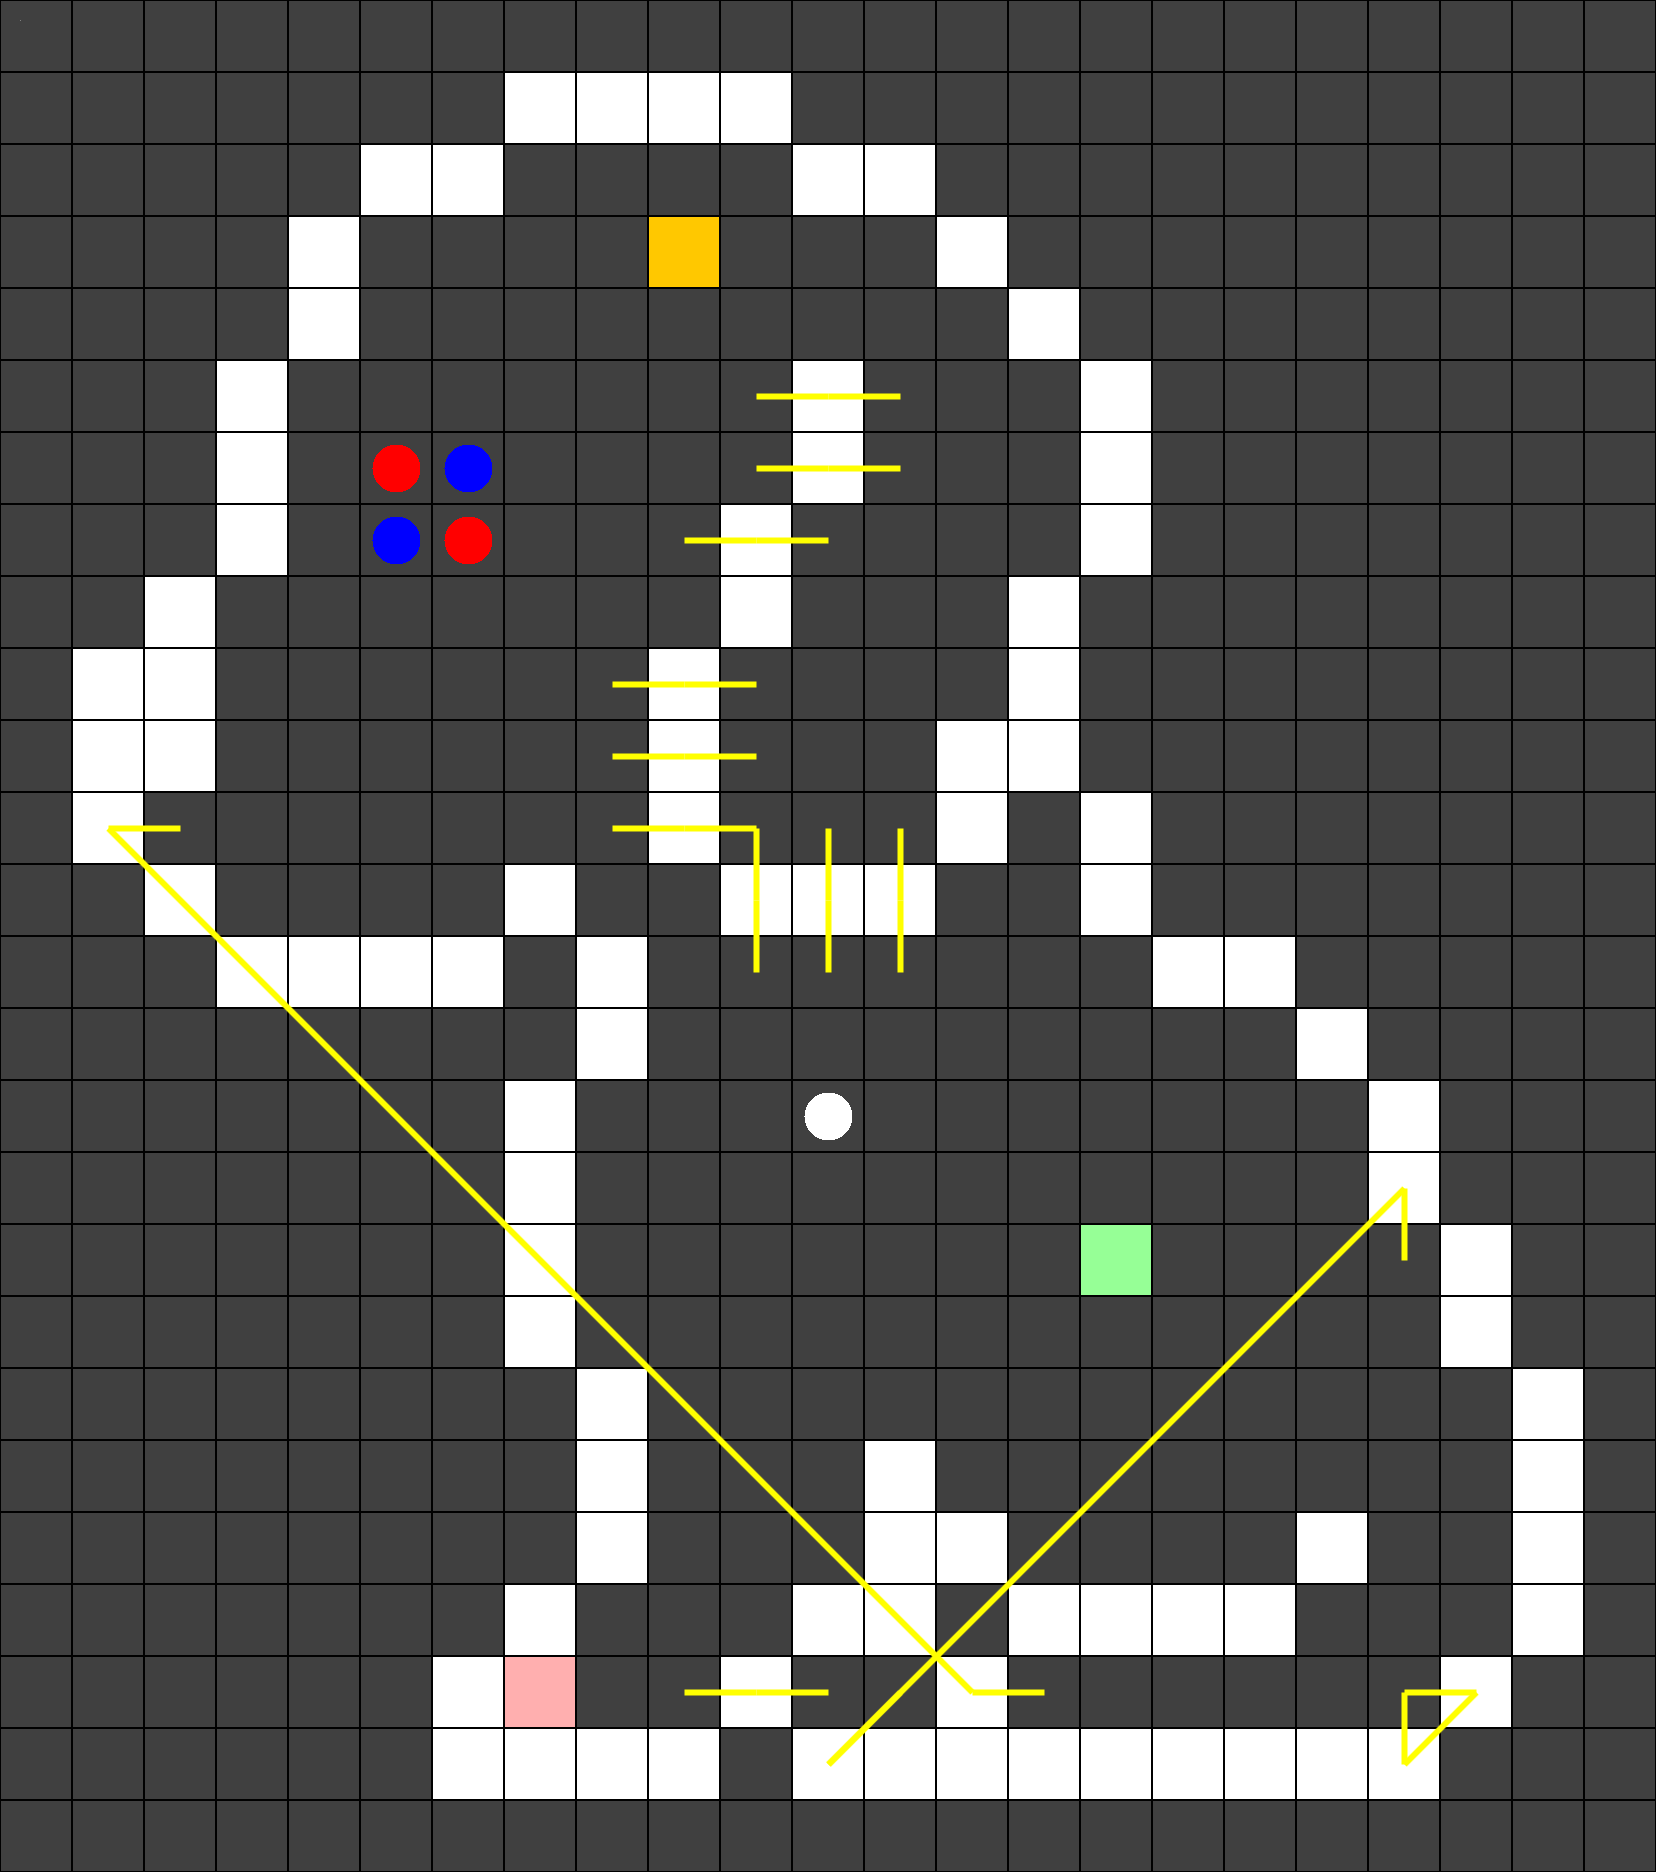
\includegraphics[width=0.4\linewidth]{pics/maps/dog-extended} }
    \qquad
    \subfloat[Karte: Europa]{ 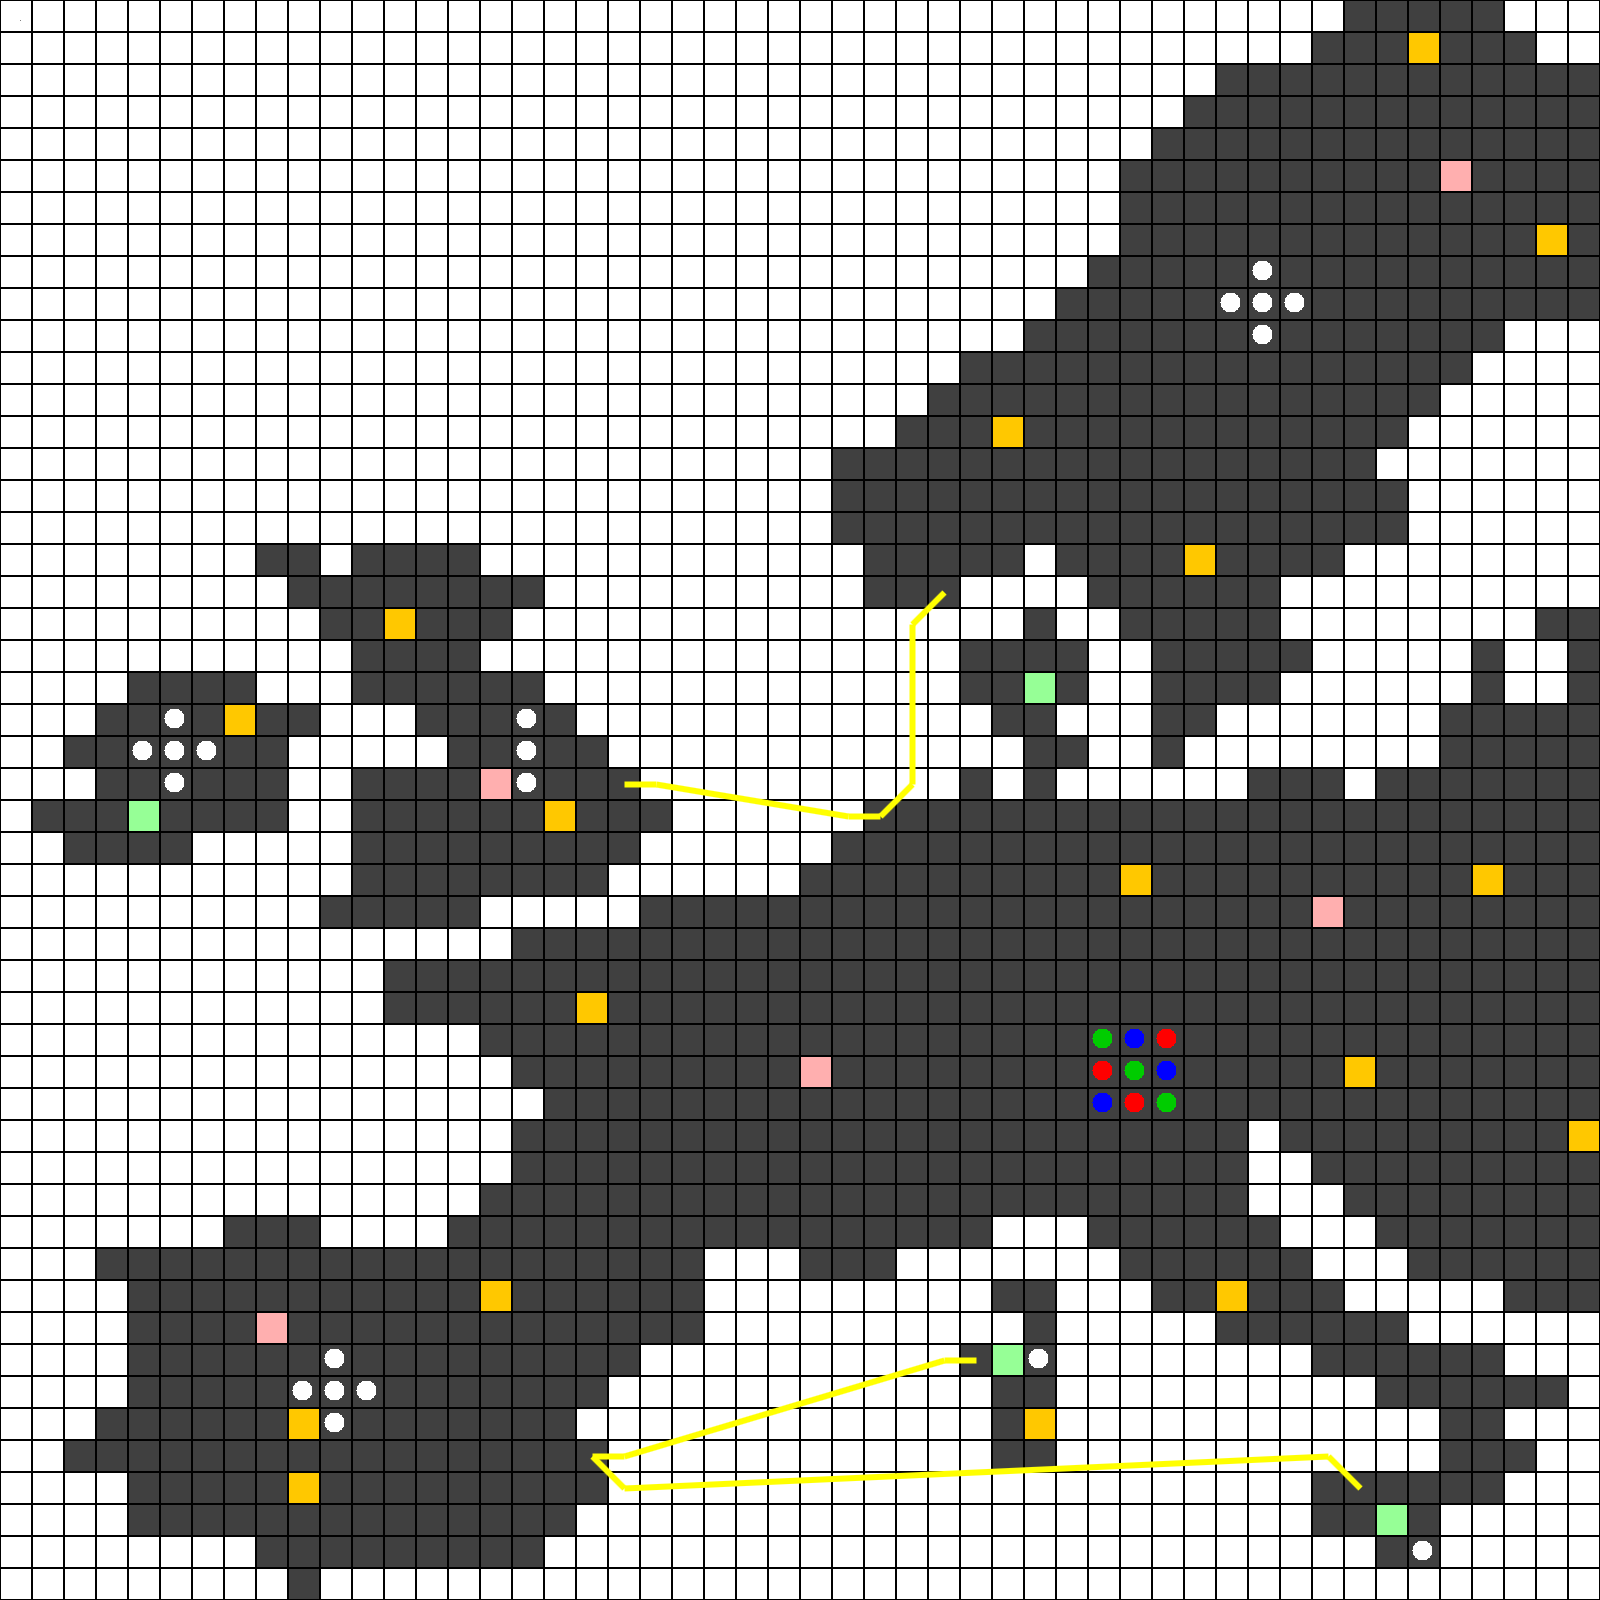
\includegraphics[width=0.5\linewidth]{pics/maps/europa} }

    \caption{Weitere Karten die f\"ur die Statistik verwendet werden}
    \label{fig:additional-statistic-maps}
\end{figure}
\vspace{1em}

\newpage

\subsubsection{Optimierung von Alpha-Beta-Pruning durch Zugsortierung}\label{subsubsec:ab-optimierung}
Wie man im Abschnitt~\ref{subsubsec:alpha-beta-pruning} gesehen hat, hilft Alpha-Beta-Pruning stark den Suchbaum zu verk\"urzen.
Jedoch wird dieser Baum bei Spielen mit mehr als zwei Spielern so gro"s, dass man hier ebenfalls auf Grenzen st\"o"st.

Eine M\"oglichkeit Alpha-Beta-Pruning zu optimieren ist, die Z\"uge vorab zu sortieren.
Die Idee besteht darin, einen vermutlich starken Zug gleich am Anfang im Suchbaum zu analysieren, um einen m\"oglichst hohen Alpha-Wert zu bekommen und dadurch alle weitern \textit{schlechteren} Z\"uge zu \"uberspringen.
Der Client sortiert also alle in seinem Spielzug m\"oglichen Z\"uge absteigend anhand der Heuristik und beginnt mit dem laut der Heuristik st\"arksten Zug.

Die Graphik~\ref{fig:sorting-01} verdeutlich was damit gemeint ist.
Man sortiert hier als blauer Spieler die Z\"uge so, dass der gr\"un markierte Zug zuerstes betrachtet wird.
Dieser ist n\"amlich besonders stark, weil man durch ihn eine Ecke gewinnt.
Somit ist hier der \texttt{MapValue} ($\equiv$ Spielfeldgewichtung) am Gr\"o"sten, da Ecken eine sehr hohe Bewertung besitzen.
Zudem gewinnt man zwei neue Steine, wodurch die \texttt{CoinParity} ($\equiv$ Spielfeldbelegung) steigt.
Dies reicht aus, um einen hohen Alpha Wert zu bekommen und im Suchbaum die schlechten Z\"uge zu \"uberspringen.

\vspace{1em}
\begin{minipage}{\linewidth}
    \centering
    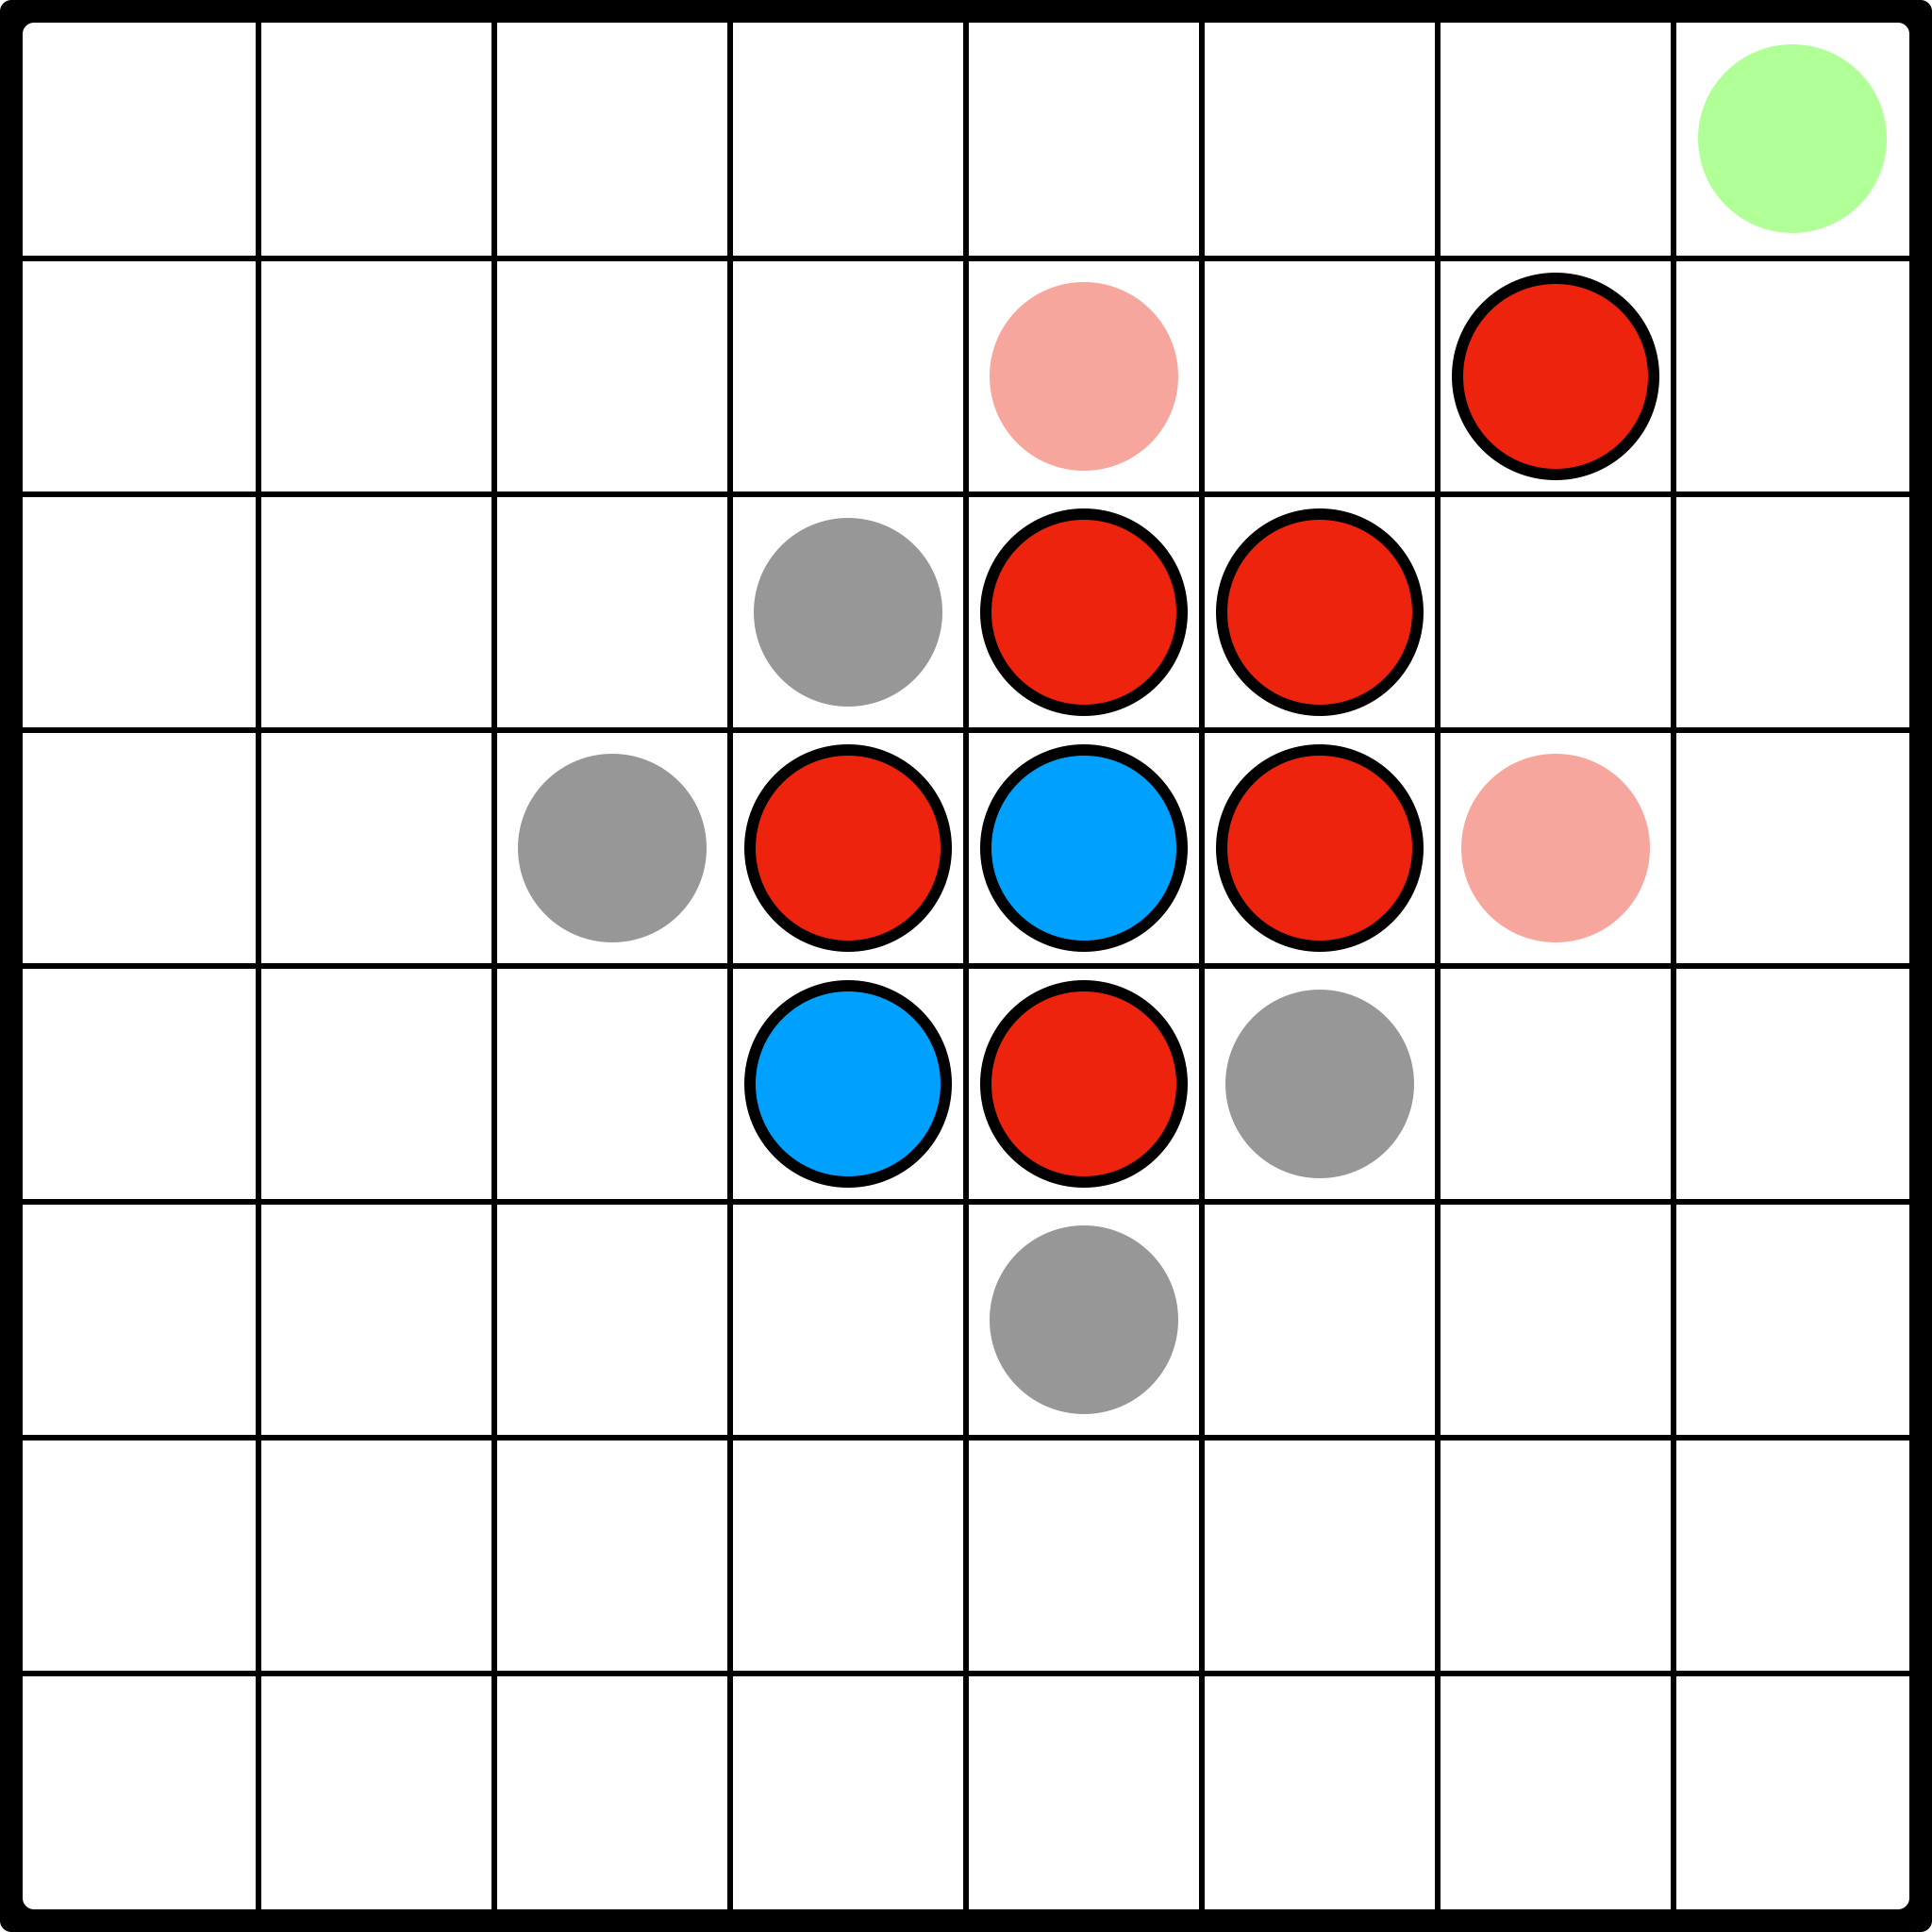
\includegraphics[width=0.45\linewidth]{pics/sorting-01}
    \captionof{figure}[Zugsortierung 01]{M\"ogliche Z\"uge f\"ur Spieler blau sortiert in unterschiedlichen Farben.}
    \label{fig:sorting-01}
\end{minipage}

Die zwei rot markierten Z\"uge betrachtet man als letztes, da beide Z\"uge genau ein Feld von der Kante entfernt sind und dadurch einen negativen MapValue haben.
Dies sollte den Client davon abhalten dort hinzuziehen und das Risiko einzugehen, die Kante an den Gegner zu verlieren.

Die Zugsortierung hat jedoch auch Nachteile, die sich aus den Nachteilen der Spielfeldgewichtung aus~\ref{subsubsec:gewichtung-des-spielfeldes} ergeben.
Wenn man n\"amlich auf einer gro"sen Karte spielt und es nur wenige Ecken und Kanten gibt dann sind die meisten Felder mit einer Gewichtung von $0$ bewertet.
Somit sind alle Z\"ugen vom MapValue gleich und unterscheiden sich nur durch die CoinParity und \texttt{Mobility} ($\equiv$ Mobilit\"at).
Wobei hier auch oft viele Z\"uge die gleichen Werte haben.
Da dieser Fall doch h\"aufig auftritt, sucht man oft ohne der Hilfe der Zugsortierung.

\subsubsection{Erweiterte Zugsortierung}
Die erweiterte Zugsortierung soll helfen das Problem der normalen Zugsortierung zu l\"osen und eine bessere Unterscheidung f\"ur vermutlich gute und schlechte Z\"uge zu liefern.
Deswegen wurde eine komplett neue und unabh\"angige Heuristik f\"ur die Zugsortierung entwickelt.

Wenn man sich die Z\"uge in ReversiXT anschaut, dann gibt es nur zwei Zugarten.
Die erste Art verdeutlich Abbildung~\ref{fig:move-move-01}.
Der blaue Spieler kann nicht ziehen, das ist jedoch nicht schlimm, weil egal welchen Zug der Rote macht, der Blaue hat immer eine Antwort, die ihn gewinnen l\"asst.
Der Grund daf\"ur ist, dass der blaue Spieler hat einen Stein an beiden Enden der Spielstein-Linie.
Dadurch kann er die Z\"uge von Rot immer kontern.
Der Blaue hat die volle Kontrolle \"uber diese Art von Anordnung.
Abildung~\ref{fig:move-simulation-01} zeigt eine im Grunde \"ahnliche Situation zu Abbildung~\ref{fig:move-move-01}.
Der Rote kann hier ebenfalls nicht gewinnen, egal wie er zieht, solange der Blaue ihn kontert.
Der Grund hierf\"ur ist wieder, dass der Blaue an beiden Enden der Linie seine Spielsteine hat.
Es ist auch egal wie die anderen Spielsteine innerhalb der Linie angeordnet sind und wie sie variieren.
Wenn man das Ganze aus der Sicht des roten Spielers betrachtet, dann sollte man Z\"uge, die zu dieser Kategorie geh\"oren vermeiden, da man in jedem Fall ein Verlust erleidet, zumindest wenn der Blaue richtig darauf reagiert.

\vspace{1em}
\begin{figure}
    \centering
    \subfloat{ 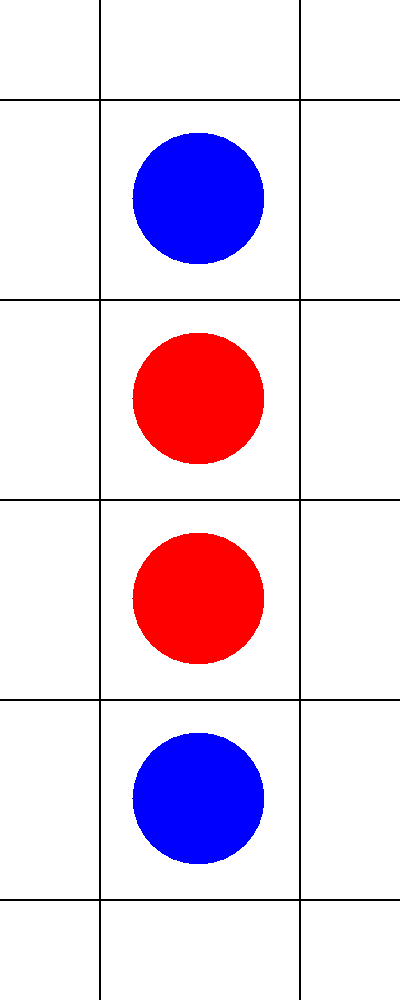
\includegraphics[width=0.1\linewidth]{pics/move-01}\label{fig:move-move-01} }
    \qquad
    \subfloat{ 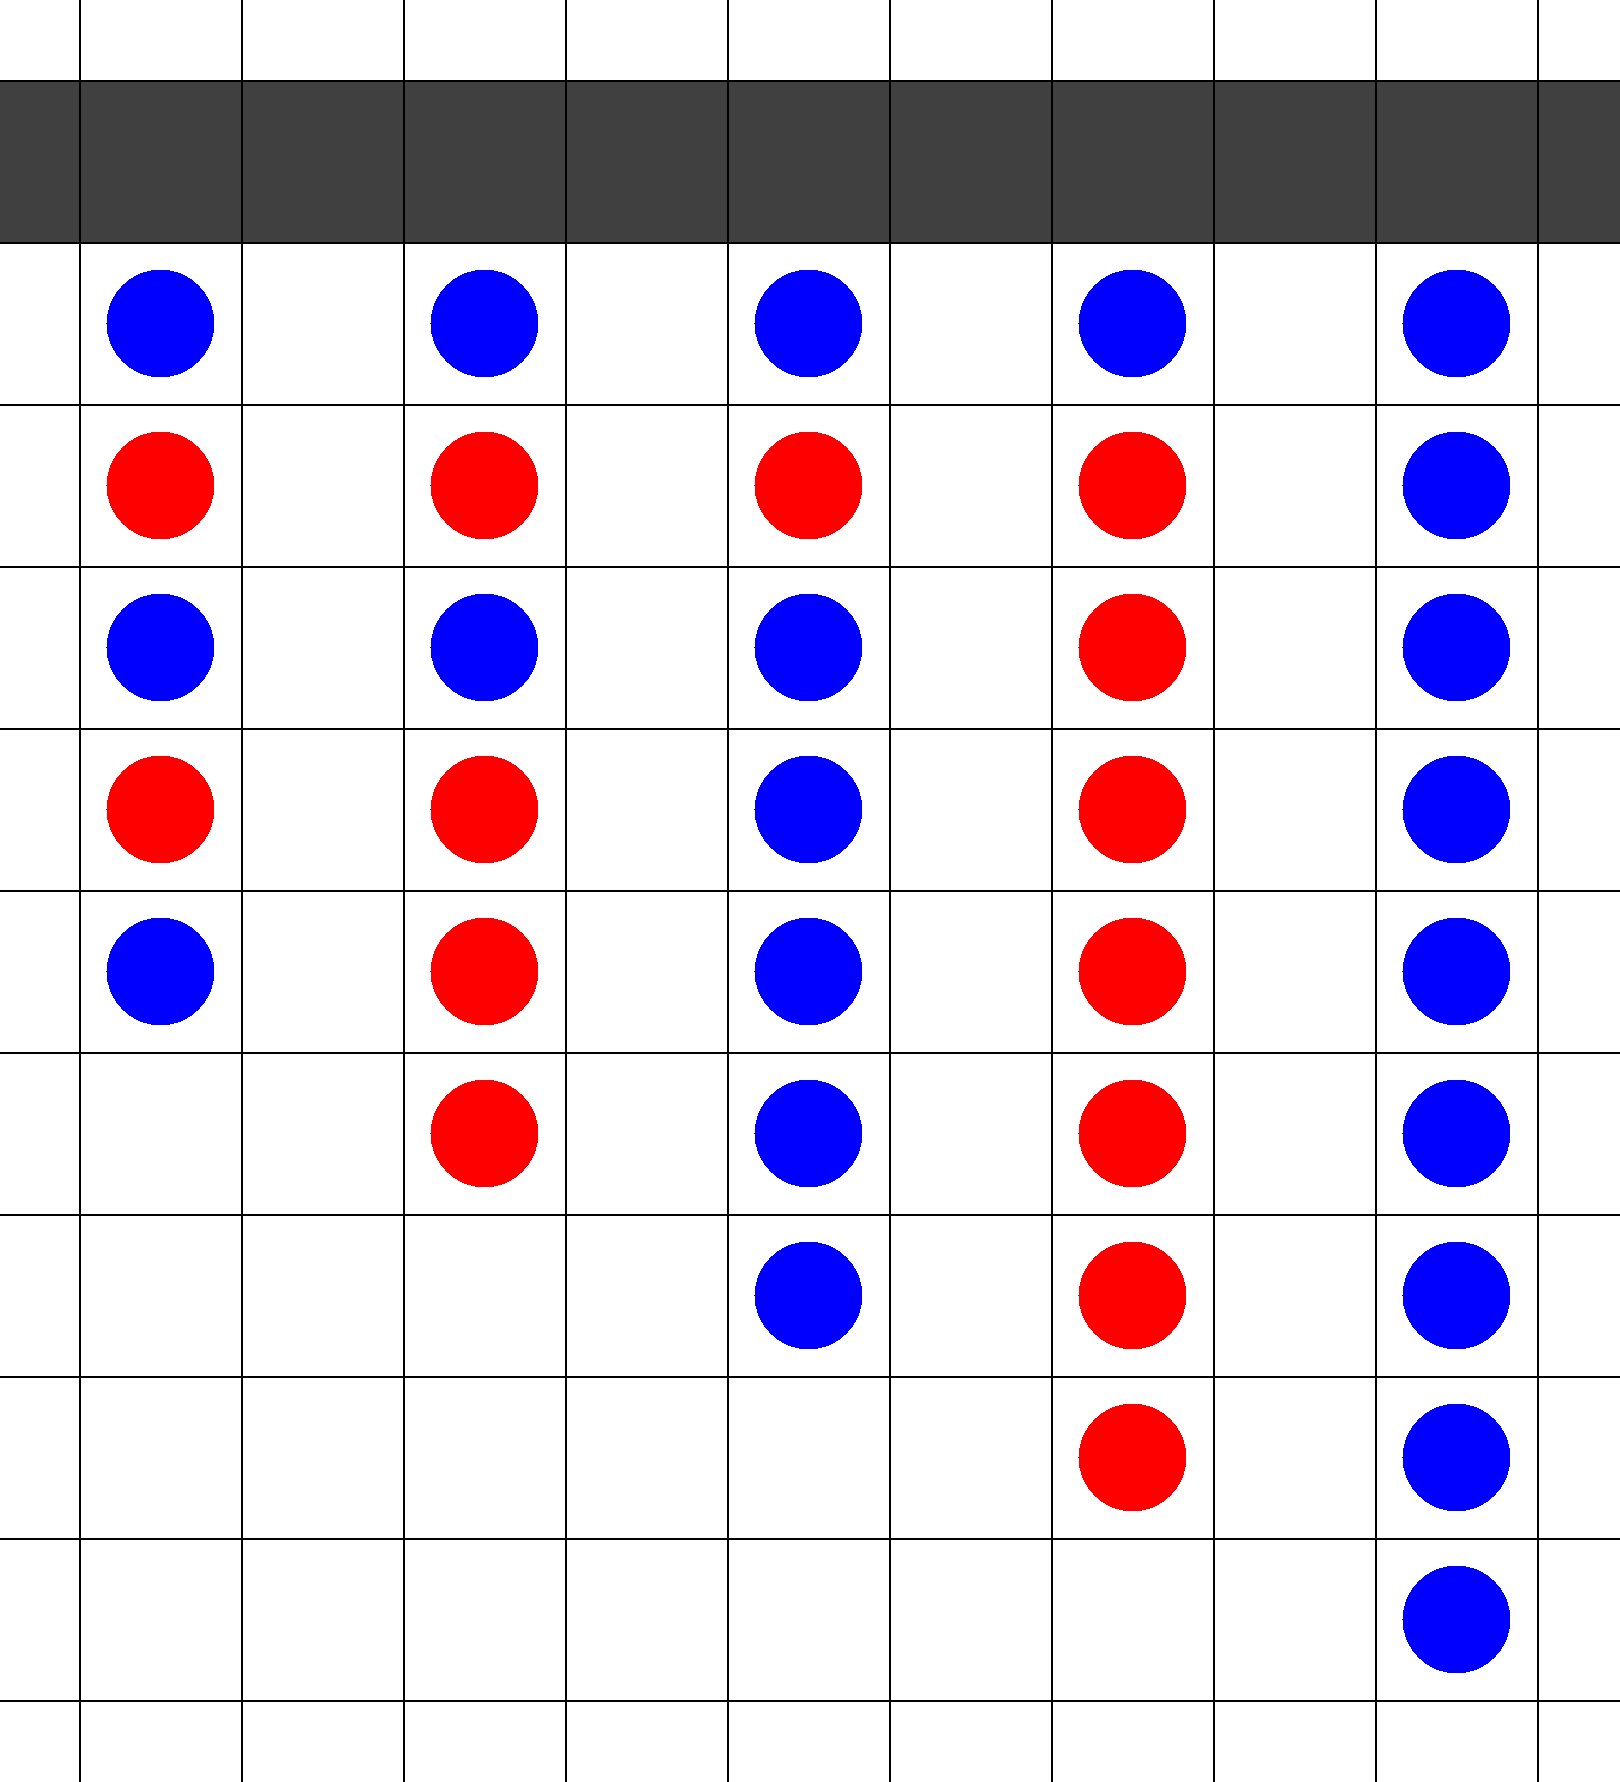
\includegraphics[width=0.3\linewidth]{pics/move-simulation-01}\label{fig:move-simulation-01} }
    \caption{Simulation eines Spielverlaufes.}
\end{figure}

Abbildung~\ref{fig:move-move-02} zeigt die n\"achste Situation.
Hier ist es stark davon abh\"angig wer ziehen darf.
Derjenige der anf\"angt wird die Situation f\"ur sich entscheiden k\"onnen und \"uberf\"uhrt die Anordnung zu einer wie in Abbildung~\ref{fig:move-move-01} oder Abbildung~\ref{fig:move-simulation-01} beschrieben wurde.
Abbildung~\ref{fig:move-simulation-02} ist ebenfalls die gleiche Situation, hier ist nur wichtig das an beiden Enden der Spielstein-Linie unterschiedliche Steine sind.

\vspace{1em}
\begin{figure}
    \centering
    \subfloat{ 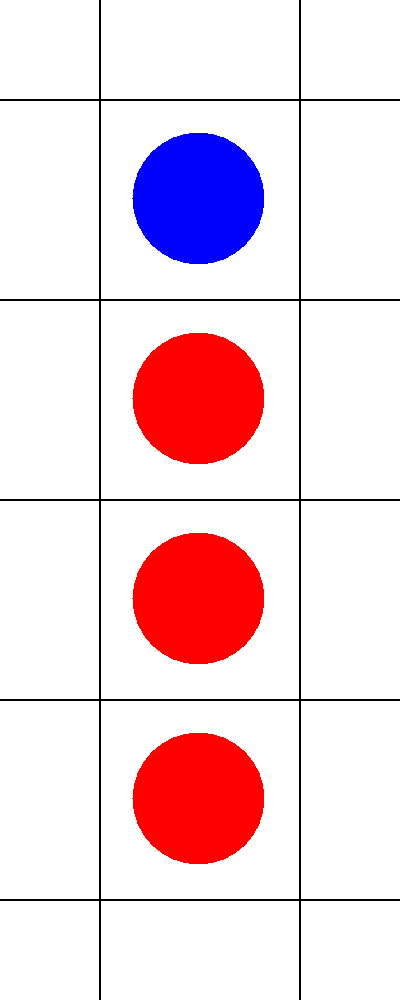
\includegraphics[width=0.1\linewidth]{pics/move-02}\label{fig:move-move-02} }
    \qquad
    \subfloat{ 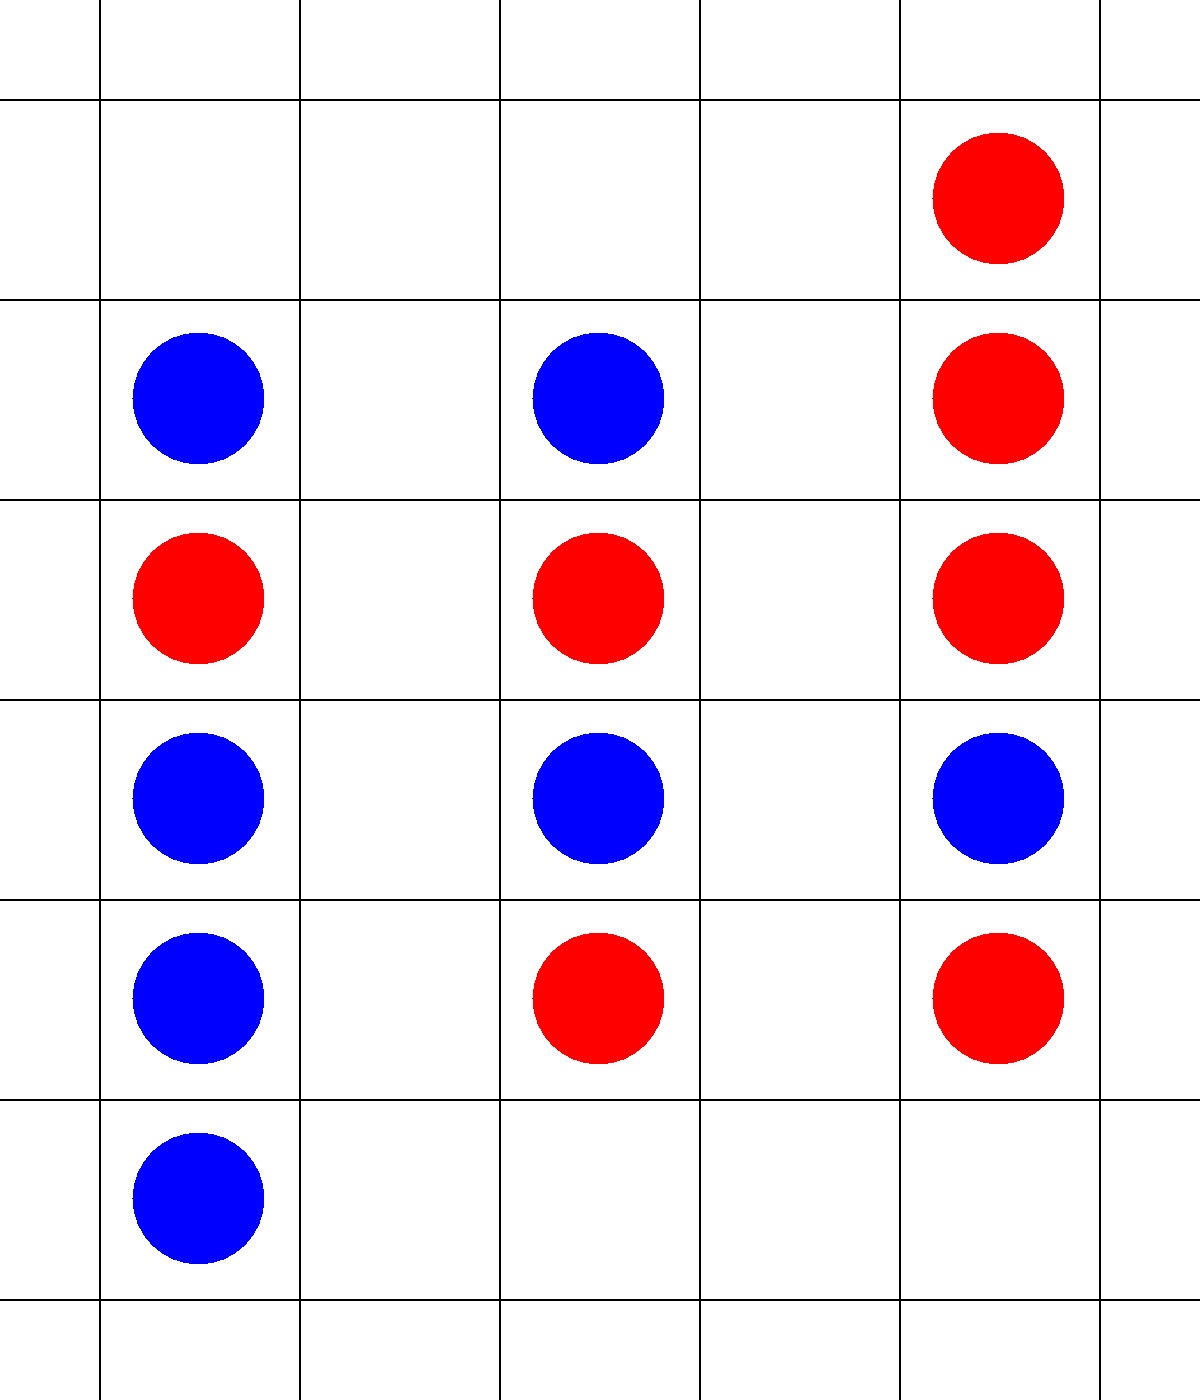
\includegraphics[width=0.3\linewidth]{pics/move-simulation-02}\label{fig:move-simulation-02} }
    \caption{Simulation eines Spielverlaufes.}
\end{figure}

Der Client teilt also die Z\"uge vorerst in die Zwei Kategorien \textit{sicherere} und \textit{unsicher} Z\"uge ein.

Die Abbildung~\ref{fig:sorting-02} zeigt, wie der Client f\"ur Spieler blau die Z\"uge kategorisieren w\"urde.
Die gr\"un markierten Z\"uge sind somit alle \textit{sicher} und die schwarzen \textit{unsicher}.
Im Suchbaum w\"urde man also nur noch die drei gr\"unen Z\"uge anschauen und die vier schwarzen Z\"uge komplett weglassen.
Das reduziert die Breite des Baumes am st\"arksten, weil bereits in Tiefe $0$ des Suchbaumes Knoten weggelassen werden.

\vspace{1em}
\begin{minipage}{\linewidth}
    \centering
    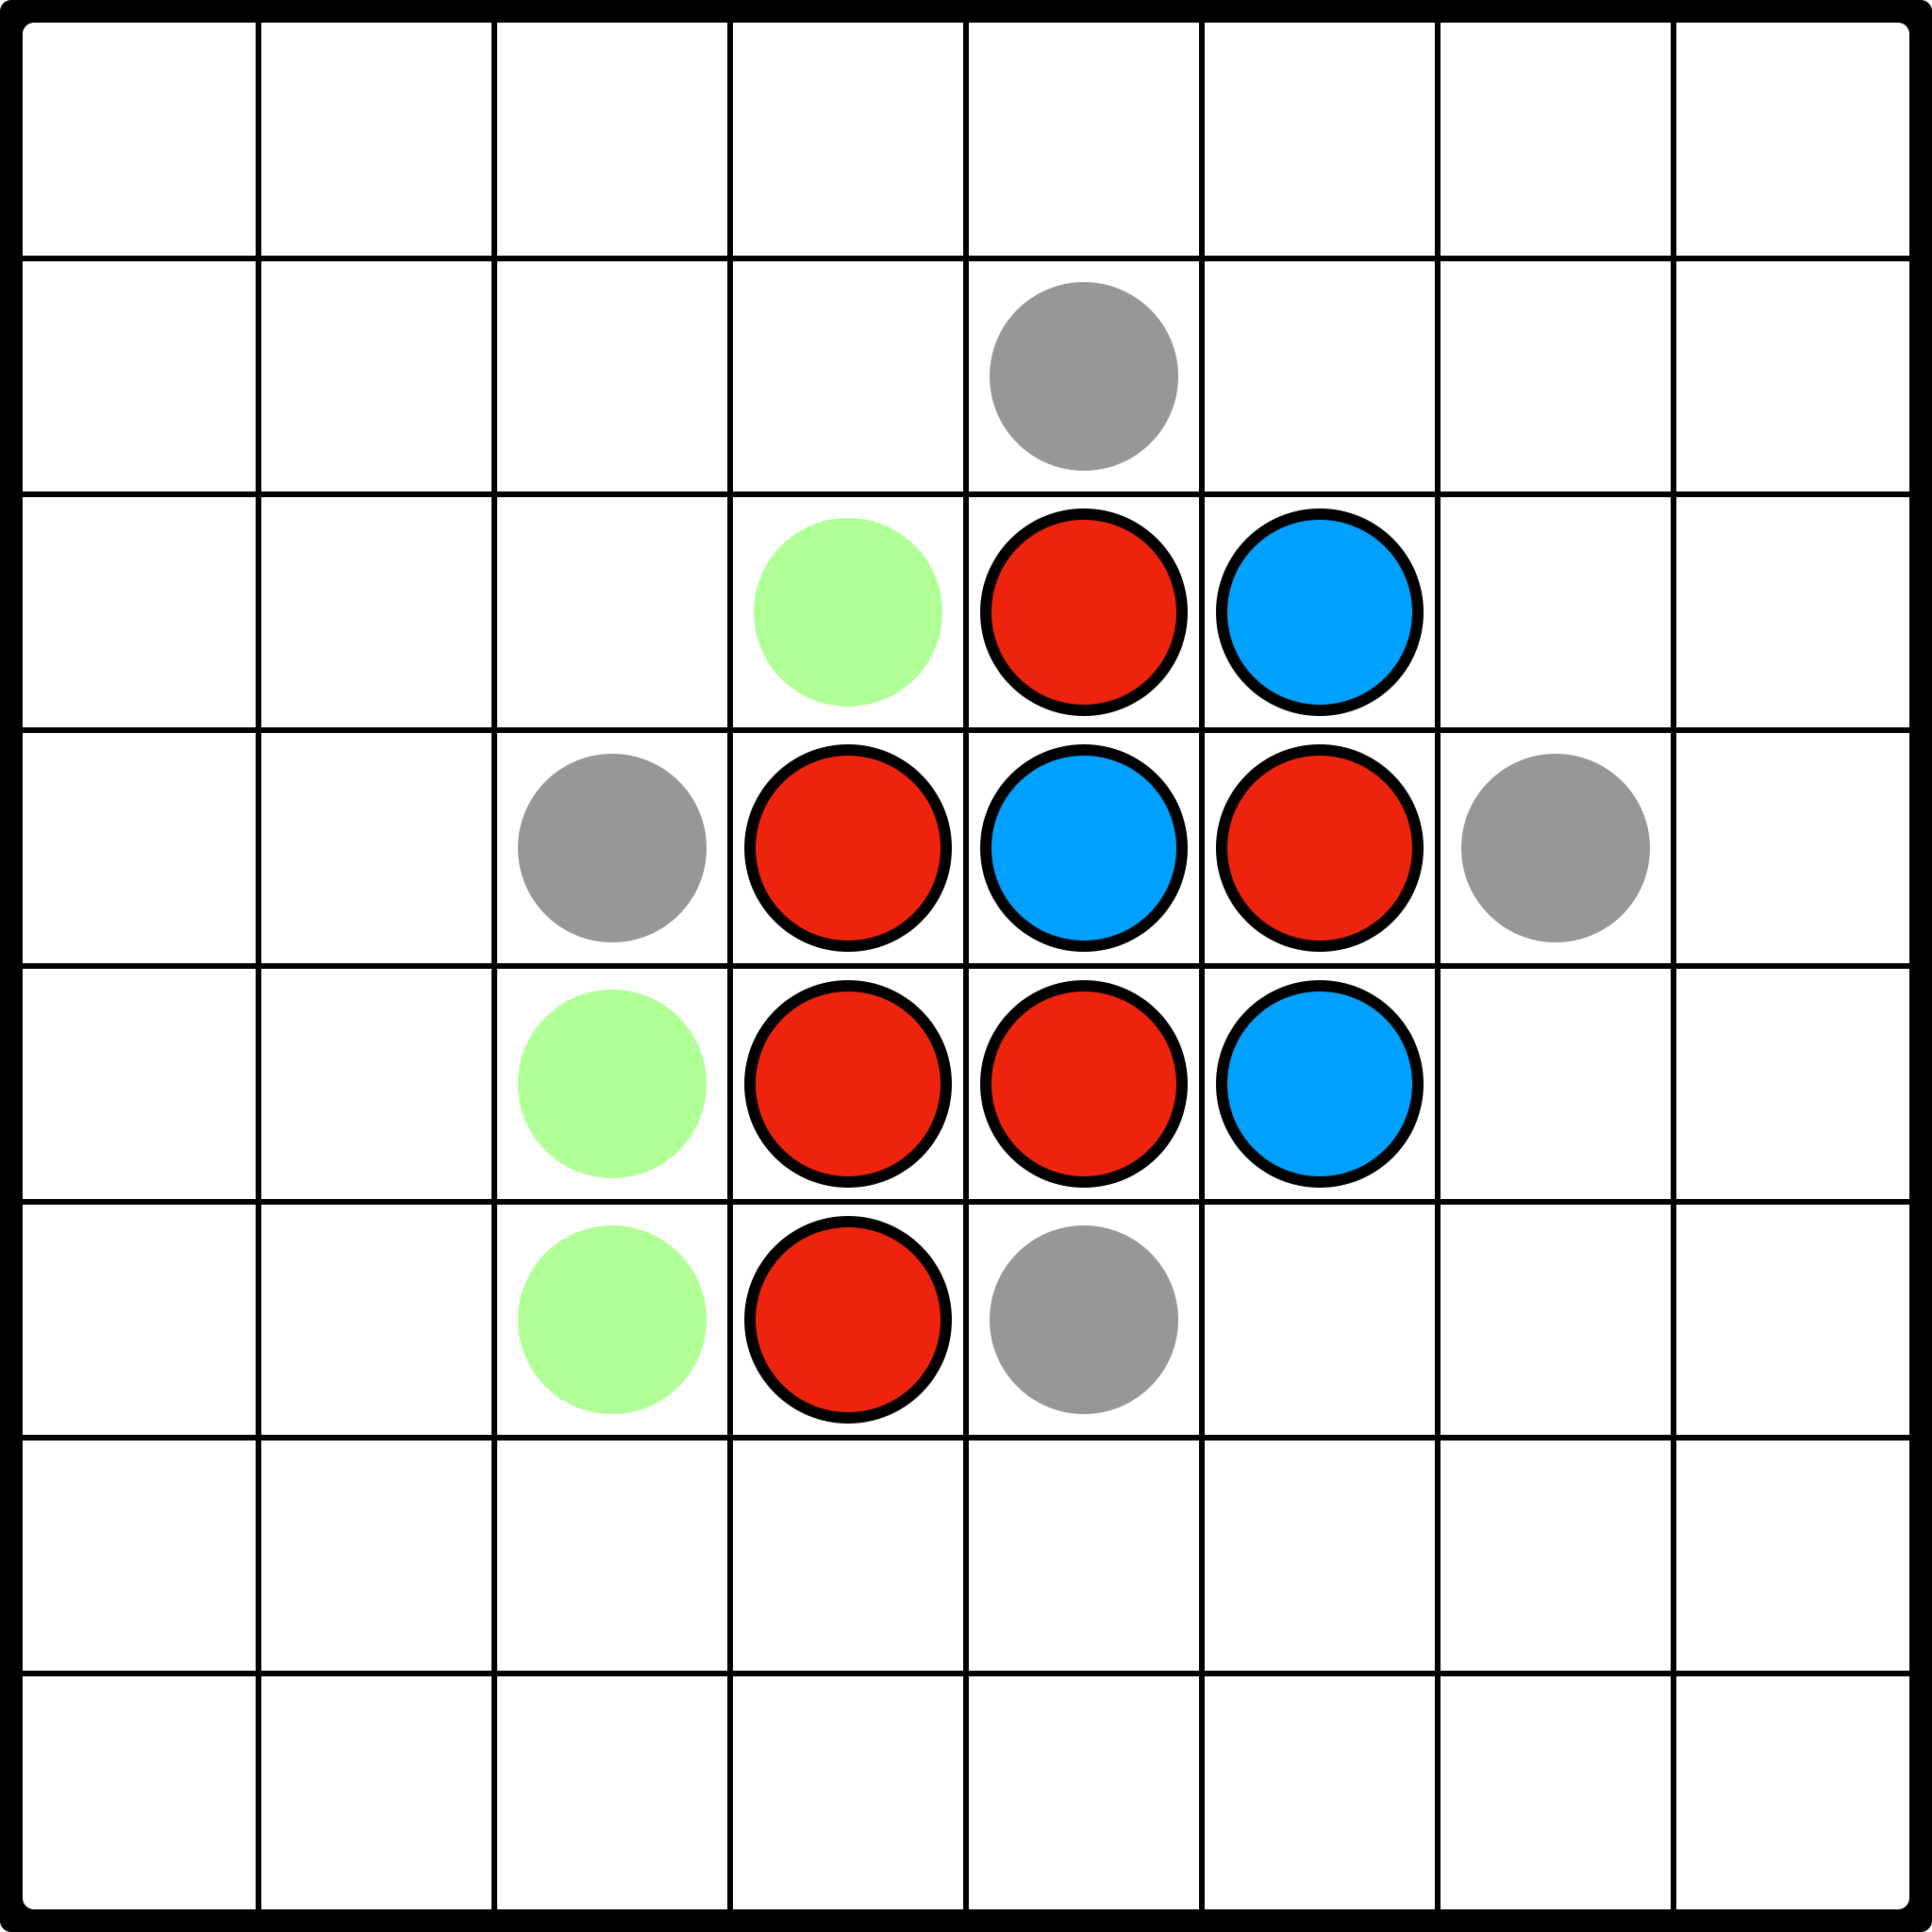
\includegraphics[width=0.45\linewidth]{pics/sorting-02}
    \captionof{figure}[Zugsortierung 02]{M\"ogliche Z\"uge f\"ur Spieler blau sortiert in unterschiedlichen Farben.}
    \label{fig:sorting-02}
\end{minipage}

Die Einteilung in \textit{sicher} und \textit{unsicher} Z\"uge wurde jedoch noch auf folgende Kategorien weiter verfeinert:
\begin{itemize}
    \item Eck-Z\"uge: Alle Z\"uge die in eine Ecke f\"uhren.
        Diese sind ebenfalls sehr sicher, da sie nur mit einem \"Uberschreibstein zur\"uckerobert werden k\"onnen.
        D.h. auch wenn am anderen Ende ein gegnerischer Spielstein ist, kontrolliert man die Situation trotzdem.
    \item Kanten-Z\"uge: Alle Z\"uge die in ein Kante f\"uhren.
        Z\"uge, die entlang einer Kante gehen z\"ahlen nicht dazu.
        Diese Z\"uge sind vorerst auch sicher, da sie in Zugrichtung nicht mehr erobert werden k\"onnen, au"ser der Gegner benutzt einen \"Uberschreibstein.
        Diese sind aber schw\"acher als Eck-Z\"uge, da sie durch normale Spielz\"uge entlang der Kante erobert werden k\"onnen.
        Das ist bei Eck-Z\"ugen nicht m\"oglich.
    \item Gefangene-Z\"uge: Sind alle Z\"uge die eine Situation wie in Abbildung~\ref{fig:move-move-01} entstehen lassen.
        Man ist also gefangen zwischen zwei gegnerischen Steinen und sollte aus dieser Situation im n\"achsten Zug nicht mehr herausziehen.
        Der Gegner kann jedoch in der Zugrichtung nicht mehr angreifen.
    \item Gute-Z\"uge: Sind alle Z\"uge, die zu Situationen wie in Abbildung~\ref{fig:move-move-01} oder Abbildung~\ref{fig:move-simulation-01} f\"uhren.
        Man hat danach also die Kontrolle \"uber den Gegner, zumindest nur in der Zug\-rich\-tung.
    \item Schlechte-Z\"uge: Sind alle Z\"uge die vorher als \textit{unsicher} beschrieben wurden.
        Also Z\"uge die vollst\"andig gekontert werden k\"onnen.
\end{itemize}
\vspace{1em}

Ausnahmen bilden Z\"uge bei denen man einen Bonus-, Choice- oder Inversionstein bekommt.
Diese Z\"uge werden unabh\"angig von den beschriebenen Kategorien betrachtet.
Bonussteine werden immer sofort genommen, wenn das im aktuellen Zug m\"oglich ist.
Choicesteine werden ebenfalls sofort ausgel\"ost.
Die Heuristik ermittelt dann anhand des MapValues, der CoinParity und der Mobility den besten Spieler mit dem getauscht werden soll.
Inversionsteine werden nur genommen, wenn die Bewertung des getauschten Spielers mindestens zu 95\% der aktuellen eigenen Bewertung entspricht.

\subsubsection{Harmlose Gegner}
In ReversiXT gibt es manchmal die Situationen, dass man am Anfang des Spiels erst nur gegen einen Spieler k\"ampft und nur im Laufe des Spiels auf andere trifft.
Ein Beispiel hierf\"ur zeigt Abbildung~\ref{fig:gitlab}.

\vspace{1em}
\begin{minipage}{\linewidth}
    \centering
    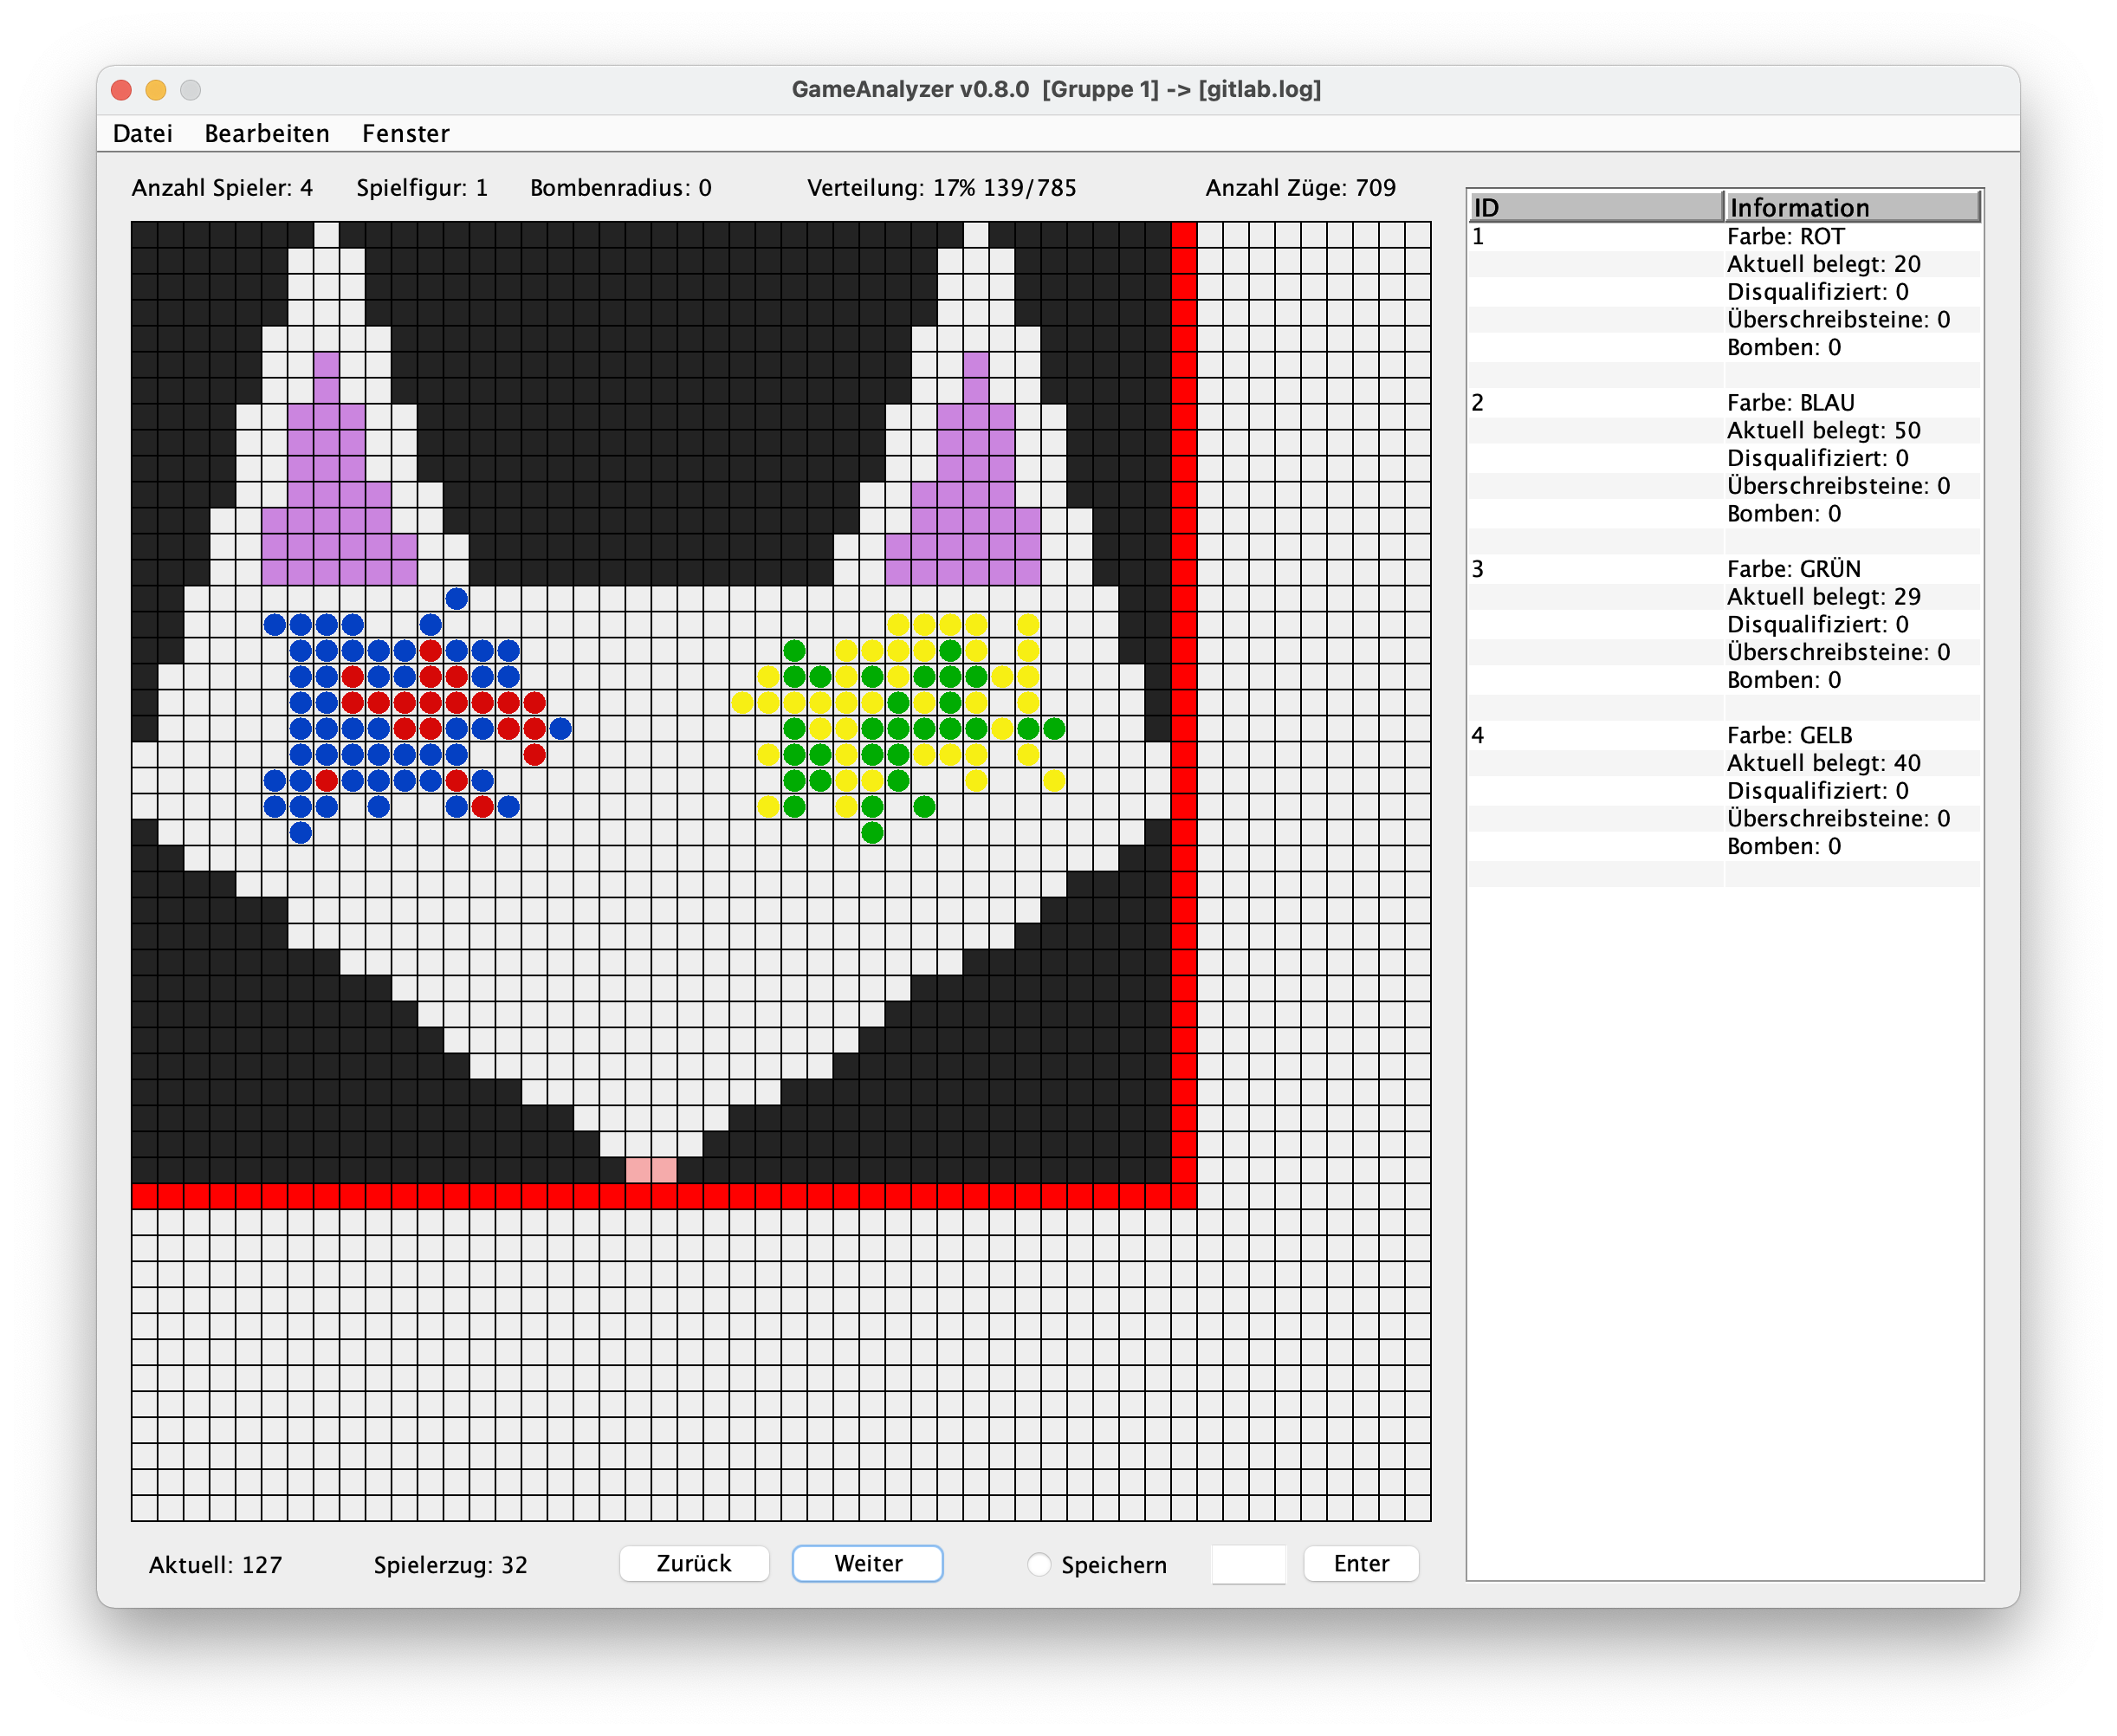
\includegraphics[width=0.8\linewidth]{pics/gitlab}
    \captionof{figure}{Spiel mit zwei vor\"ubergehenden unabh\"angigen Spielen}
    \label{fig:gitlab}
\end{minipage}
\vspace{1em}

Auf dieser Karte startet man in zwei Gruppen und wird erst sp\"ater auf andere treffen.
F\"ur den Suchbaum macht es also keinen Sinn, alle Z\"uge vom Gegner zu betrachten die aktuell gar nicht die eigenen Spielsteine angreifen k\"onnen.
In solchen Situationen kann man also die vorerst \textit{harmlosen} Gegner im Suchbaum \"uberspringen, in dem man von ihnen nur einen zuf\"alligen Zug ausf\"uhrt.
Durch diese Taktik reduziert man quasi den Baum nur auf Gegner die einen direkt betreffen.

Diese Optimierung funktioniert jedoch nicht mehr, wenn alle Gegner einen angreifen k\"onnen.


\bigskip
\newpage